

\newcommand{\qq}[2]{\emph{``#1"} (#2)}
\newcommand{\HAtheme}[2]{\textbf{Theme #1:} \uline{#2}\\}



\chapter{Refine: Tactile Animation}
\label{ch:tactileanimation}

  % \teaser{
\begin{figure}[h]
   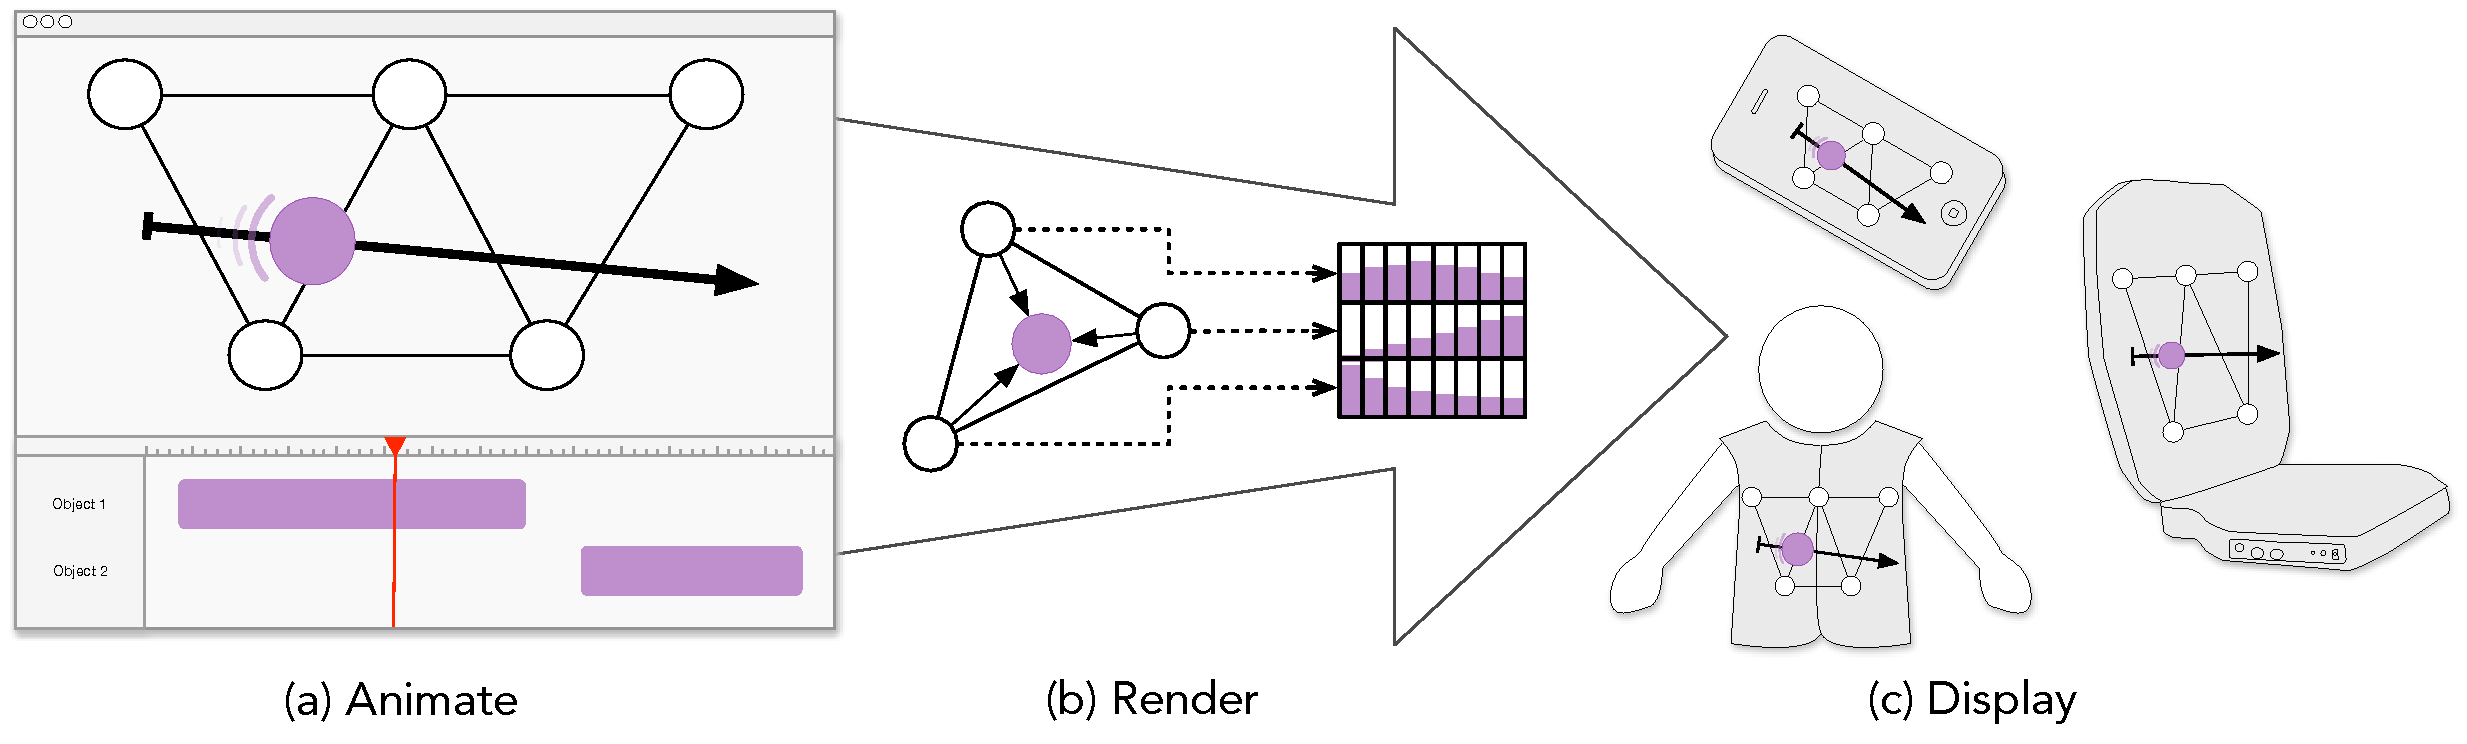
\includegraphics[width=0.98\textwidth]{images/HA14-Concept-Sketch-2015-01-17-1127}
   \caption{Concept sketch for tactile animation. 
An artist draws an animated sequence in the user interface and the user experiences phantom 2D sensations in-between discrete actuator grids. 
%The animator controls phantom sensations directly, without needing to think in device terms, and designs expressive sensations for arbitrary vibrotactile arrays.
}
   \label{fig:concept:sketch}
\end{figure}
% }

  

%Chairs, wearables, and handhelds have become popular sites for spatial tactile display.
%Visual animators, 
%already expert in using time and space to portray motion, could readily transfer their skills to production of rich haptic sensations if given the right tools.
\noindent
\inlineHeading{Preface} In this second case study\footnote{\fullCitation{Schneider2015}}, we iterate on our findings from the haptic instrument to build a full authoring tool that supported both \emph{sketching} and \emph{refinement}.
This work expanded to spatial vibrotactile designs with professional non-haptic media designers.
We surveyed critical haptic authoring tool features and developed a full rendering pipeline for the tactile animation object, an abstraction able to handle diverse spatial vibrotactile arrays. %We describe Mango's interface, rendering pipeline, and perceptually-optimized interpolation algorithm.
We evaluated the implemented tool, Mango, with both phenomenology and methods from grounded theory and iterated on our study tasks.
Professional animators transferred their non-haptic design skills to both explore (sketch) and iterate (refine), but missed features to reuse design elements and gather inspiration from examples.
This theme, also glimpsed in \autoref{ch:hapticinstrument}, lead to the third design activity: \emph{browse}.
%Furthermore, the tactile animation metaphor is a generalizable concept that can extend to several devices.
%, which we explore before concluding.
%in authoring real-time feedback on a variety of grid displays.

%Tactile Animation let us
%\osC{TODO: prosify this additional framing, outline chapter.}
%  - develop a full pipeline editing tool
%  - ground our designs in industry concerns
%  - evaluate with non-haptic media designers to investigate transfer effects
%  - expand our design palette to spatial vibrotactile effects, unexplored directly in the haptic instrument case study
%  - in particular, we expand to a directly-manipulated metaphor
%  - look at device generality in a different way than the haptic instrument. In the haptic instrument, one can build a haptic instrument for new output devices by connecting nput parameters to different output devices. Here we look at a class of devices - 2D vibrotactile grids, but possibly other 2D grids.
%   - this direct manipulation metaphor is distinguished from other spatial control by \autoref{fig:tactileanimation:prevwork}.



\section{Abstract}
Chairs, wearables, and handhelds have become popular sites for spatial tactile display.
Visual animators, 
already expert in using time and space to portray motion, could readily transfer their skills to produce rich haptic sensations if given the right tools.
%We introduce the \emph{tactile animation object}, an abstracted primitive 
We introduce the \emph{tactile animation object}, a directly manipulated phantom tactile sensation.
This abstraction has two key benefits: 1) efficient, creative, iterative control of spatiotemporal sensations,
and 2) the potential to support a variety of tactile grids, including sparse displays.
%enabling direct manipulation of phantom vibrotactile sensations continuously in space and time, and
We present Mango, an editing tool for animators, including its rendering pipeline and perceptually-optimized interpolation algorithm for sparse vibrotactile grids.
In our evaluation,
professional animators found it easy to create a variety of
vibrotactile patterns, with both experts and novices preferring the tactile animation object over
controlling actuators individually.

  
%%%%%%%%%%%%%%
%
% Section - Intro
%
%%%%%%%%%%%%%%
\section{Introduction}

Haptic feedback is
viewed today %in today's
%entertainment and media industry
as a key ingredient of immersive media experiences.
Body-moving devices in theatre seats, ride vehicles, and gaming platforms can tilt, translate, and shake the user for increased engagement. 
Recently, arrays of multiple actuators have been developed to display expressive, spatial sensations on the skin 
%aim to supplement movies, games, and social activities with expressive, synchronized cues at multiple locations 
\cite{Israr2011,Danieau2012a,Sodhi2013,Kim2009,Wilson2014}. 
%Similar opportunities await well-designed wearable and handheld displays.

Vibrotactile (VT) arrays,
which stimulate the skin through vibration, are common in diverse applications from immersive gaming chairs  \cite{Israr2011} to wearable vests for mobile awareness \cite{Jones2004}.
%To create expressive sensations, however, designers typically must be programmers and haptic experts.
%Several device-specific tools for prototyping or final authoring of haptic sensations have introduced user-friendly and user-familiar interfaces.
These displays typically employ sparse actuator arrangements to reduce cost and power requirements, using perceptual illusions to create continuous sensations \cite{Alles1970,Israr2011a,Seo2013}.
Unfortunately, adoption of VT arrays is limited by a lack of authoring tools.
Most only support a single actuator \cite{Enriquez2003}; those that accommodate multiple actuators % deleted Lee2009
control each separately \cite{Kim2009,Paneels2013,Swindells2014},
%Separate actuator control %allow designers to edit, test, and save time-series data for individual actuators, but
%supports smaller, denser arrays \cite{Kim2009} but
%can be 
cumbersome for non-adjacent actuators.
%, with as many as % greater than 
%%10 or 20 vibrating actuators (e.g., one haptic jacket for movie goers is equipped with 
%64 vibrators \cite{Jones2009}.
%%). %(Tactile 

To remedy this, we propose the \textit{tactile animation object}, an abstract, directly manipulable representation of a phantom sensation perceived in-between physical actuators.
% to support real-time spatiotemporal tactile feedback in sparse actuator arrays, enabling direct manipulation.
%{\it Direct manipulation} of a spatial animation object provides
%rather than by coordinating multiple tracks. 
With this approach, designers can 
%eases the transition of visual animators into haptic design.
efficiently and creatively explore ideas and iterate without worrying about underlying actuator arrangements.
As long as a rendering algorithm can be developed, this abstraction not only facilitates design, but is compatible with a variety of form factors and technologies.

In this paper, we describe the tactile animation object and implement it in \emph{Mango}, a tactile animation tool and pipeline (\autoref{fig:concept:sketch}).
Our contributions are: 
%We have three contributions.
1)  A tactile animation interface grounded in user interviews and prior literature.
% The design is derived from interviews and prior literature, ..  includes tools 
%Derived from interviews and prior literature, its design integrates techniques familiar to a mainstream animator workforce. 
2) A rendering pipeline translating tactile animation objects %designed % animated 
%haptic patterns to sparse VT arrays, and optimize its rendering algorithm with a user study.
to phantom sensations on sparse, generalized VT arrays, optimized with a perceptual study.
% We conduct a study to determine an optimal rendering algorithm for sparse VT arrays. 
3) An evaluation with professional animators showing accessibility and expressivity.
4) An exploration of  potential applications for tactile animation.
% with \kmC{SLC} % in  ??? 
%natural user gestures.
% KM 04.12: at this point, 'animation metaphor' as connected to 'natural user gestures' is unclear - you haven't mentioned gestures yet so this comes out of nowhere. Can you restate this contribution more plainly?

%%%%%%%%%%%%%%
%
% Section - Related Work
%
%%%%%%%%%%%%%%
\section{Background}

%%%%%%%%%%%%%%
%
% Subsection - VT perception
%
%\subsection{Haptic Icons and Vibrotactile Perception}

\subsection{Haptic Entertainment Technologies}
Haptic feedback was % has been 
used in cinema as early as \emph{Percepto}, a 1959 multisensory experience for the movie ``The Tingler"  \cite{IJsselsteijn2003} %
%G. Riva, F. Davide, and W.A. IJsselsteijn, �Presence in the Past: What Can We Learn from Media History?,� Being There: Concept, Effects and Measurements of User Presence in Synthetic Environments, IOS Press, 2003, Amsterdam, The Netherlands, pp. 17-40.
with theater seats % The theater seats were 
% equipped with vibrating devices 
that buzzed the audience at strategic moments. % during events in the movie.
Current 4D theaters, rides, shows, and gaming arcades are equipped with sophisticated motion platforms (e.g., D-Box, www.d-box.com) that supplement visual scenes. % with subtle and synchronized movements.
Large tactile transducers (such as Buttkickers, www.thebuttkicker.com) that shake the entire seat using the sound stream are also common with gaming and music content. %, therefore allowing users to feel `bumps' during musical beats and gameplay.   
Custom editors (such as D-Box Motion Code Editor) and software plugins %enable media designers that
overlay visual and audio content with haptics, and allow designers to generate, tune and save frame-by-frame haptics in an allocated track. %for simultaneously with  media content. 

In contrast to displacing the entire body, multichannel haptic devices create percepts of dynamic and localized haptic sensations on the user's skin \cite{Israr2011} and in mid-air \cite{Wilson2014}.
% and in the mid-air \cite{Wilson2014}.
Similar devices have been % are also
developed for online social interactions using custom multi-actuator displays  %haptic devices 
\cite{Kim2009,Tsetserukou2009,Paneels2013}. %Tsetserukou, D. and Neviarouskaya, A. iFeel_IM!: augmenting emotions during online communication. Comp. Graphics & Applications 30 (2009), IEEE, 72-80.
%  Designers (and researchers) for these technologies must have 
% Use of
All of these technologies require extensive programming experience, knowledge of hardware and background in haptic sciences to generate expressive and meaningful haptic content. 
% Due to the lack of
Without guiding principles or haptic libraries,  content generation schemes are complex, device-specific, and time consuming. 


Another class of haptic technology renders high-resolution spatio-temporal patterns on the skin using a sparse array of VT actuators.
These technologies use parametric models of sensory illusions in touch, such as phantom tactile sensations \cite{Alles1970}, and create illusory vibrations in between two or more VT actuators.
%For example, Seo and Choi % KM: when you give authors names in text this way, you can reduce the citation to just the year to avoid clumsy redundancy. However, while I thought there was an easily accessed bibtex citation alternative, I can't find it now. (seem to have to install natbib package and this creates other problems).
%OS: Couldn't figure this one out (biblatex is another package that causes other issues), restructured to be a little less jarring.
%
This idea has been used to % has been done to
create a perceived motion flow between two vibrators mounted on the ends of a handheld device % by controlling their intensity
\cite{Seo2013} and to
%Lee and colleagues
create across-the-body and out-of-the-body illusions on a mobile device using up to four % inexpensive 
%linear resonant 
actuators \cite{Lee2012a}.
The Tactile Brush algorithm \cite{Israr2011a} combined phantom tactile sensations and apparent tactile motion to render high-resolution and moving haptic patterns on the back using a coarse grid of VT actuators, but paths must be pre-determined (\autoref{fig:prevwork:tactilebrush}). 
Other spatio-temporal VT illusions such as the  ``cutaneous rabbit"  \cite{Tan2009} and Tau and Kappa effects \cite{Hayward2008} can be also used with VT arrays.


%Spatial displays of tactors (VT actuators) are a promising avenue for chair-based immersive gaming experiences \cite{Israr2011}, sleeves for social touch \cite{Huisman2013}, or wearable vests for mobile awareness \cite{Jones2004, Brewster2010}.%and artistic compositions \cite{Gunther2002}. Here we cover relevant work on VT communication and perception, and the literature on haptic authoring tools.

%%%%%%%%%%%%%%
%
% Subsection - Haptic authoring tools
%
\subsection{Haptic Authoring Tools}
As long as designers have considered haptic effects for entertainment media, they have needed compositional tools % to facilitate their design 
\cite{Gunther2002}.
% Much previous work has focused on how to prototype, sketch or control haptic phenomena using non-programming methods, % This section highlights those past literature and the 
Requirements drawn from previous work on how to prototype, sketch, or control haptic phenomena using non-programming methods are summarized in
% Key features of these tools are summarized in 
\autoref{tab:design:literature:requirements}.
%A thorough review of prior literature is presented below.

The Hapticon editor \cite{Enriquez2003}, Haptic Icon Prototyper \cite{Swindells2006}, posVibEditor \cite{Ryu2008}, and Immersion's Haptic Studio (www.immersion.com) use graphical representations to edit either waveforms or profiles of dynamic parameters (such as frequency or torque) over time.
%Features include the combination or multi-tracking of effects, utilizing a library of existing effects, and the ability to play back sensations.
Another %popular trend has been to augment  media content with 
approach is predefining a library of haptic patterns to augment media content. %during the development process.
Immersion Corporation's Touch Effects Studio lets users enhance a video from a  library of tactile icons supplied on a mobile platform.
Vivitouch Studio \cite{Swindells2014} allows for haptic prototyping of different effects alongside video (screen captures from video games) and audio. 
These tools focus on low-level control of device features rather than a semantic space, and control devices with either a spatial or temporal component, but not both simultaneously. 




\newcommand\prevWorkWidth{1.25in}
\newcommand\prevWorkImageWidth{1.1in}


\begin{figure}[t]
 \centering
   \begin{subfigure}[t]{\prevWorkWidth}
	  \centering
	   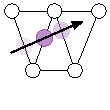
\includegraphics[width=\prevWorkImageWidth]{HA14-PreviousWork-TactileBrush-2015-04-12-1100} 
	   \caption{Tactile Brush \cite{Israr2011a}: precomputed paths}
	   \label{fig:prevwork:tactilebrush}
    \end{subfigure}
    \qquad
  \begin{subfigure}[t]{\prevWorkWidth}
  	\centering
	   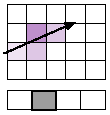
\includegraphics[width=\prevWorkImageWidth]{HA14-PreviousWork-TactileMovies-2015-04-12-1100} 
	   \caption{Tactile Video \cite{Kim2009}: frames of tactile pixels}
	   \label{fig:prevwork:tactilemovies}
    \end{subfigure}
	\qquad
      \begin{subfigure}[t]{\prevWorkWidth}
	      \centering
	   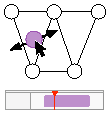
\includegraphics[width=\prevWorkImageWidth]{HA14-PreviousWork-HA-2015-04-12-1100} 
	   \caption{Tactile Animation: direct manipulation}
	   \label{fig:prevwork:ha}
    \end{subfigure}
    \caption{Comparison between related systems.}
    \label{fig:tactileanimation:prevwork}
\end{figure}




\begin{table*}
	\begin{tabular}{|l|p{0.92\textwidth}|}
	\hline
	\rowcolor{tableheadercolor}

	\textbf{LR}
		%& \textbf{RW}
		& \textbf{Description} \\
	\hline
		LR1 
		 &
		 \textbf{Real-Time Playback} \cite{Moussette2011,Schneider2014}
		 Rapid prototyping is essential for working with VT sensations, especially in absence of objective metrics. % of success.
		 Feeling a sensation at design time allows iteration to converge faster to better results. % and develop more engaging sensations.
		 However, \textit{too} real-time can cause split attention.
	\\
	\hline
		LR2 & 
		 \textbf{Load, save, manipulate}
		 \cite{Resnick2008,Johnson2002,Schneider2014}
		 	A persistent object model is essential for sensation editing over % for being able to continue to work on sensations for 
			longer projects and % for being able to share them 
			sharing with other designers or across devices.
			Well-defined actions upon a data structure also facilitates features like \textit{undo} that support experimentation.
	\\
	\hline
		LR3 &
		\textbf{Library of effects} \cite{Enriquez2003,Swindells2006,Herring2009,Paneels2013,Swindells2014}
		% deleted Paneels2010
			 A library of saved sensations is an important feature used in previous haptic authoring tools, providing inspiration and preventing designers from re-inventing the wheel.
	\\
	\hline
		LR4 &
		\textbf{Device configuration} \cite{Kim2009,Paneels2013,Lee2012,Lee2013}% deleted Lee2009
			~Because of the many types of haptic devices, a general tool must be able to understand different devices.
			Lightweight configuration files are common in the literature, allowing users to select specific hardware, specify location and type of actuators, and choose a rendering algorithm.
%			Animators can also select a rendering algorithm from a list of available ones.
	\\
	\hline
		LR5 &
		\textbf{Multiple channels \& combination of effects}
		 \cite{Enriquez2003,Swindells2006,Ryu2008,Paneels2013,Swindells2014}	 
		 Being able to display multiple effects simultaneously, or combine effects via superposition or concatenation, is essential for expanding the design space.
		 This is typically represented in a timeline, which represents the temporal behaviour of any objects.
	\\
	\hline
		LR6 &
		\textbf{Visual/direct control metaphor}
		\cite{Kim2009,Paneels2013,Cuartielles2012}
		 Most previous tools consider each actuator separately.
		 When thinking semantically about a spatial system, a direct view of the device and actuator layout is critical for direct manipulation.
	\\
	\hline
		LR7 &
		\textbf{Audio/visual context}
		\cite{Kim2009,Swindells2014,Moussette2011}
		 Haptic perception depends greatly on additional senses \cite{Hayward2008}. %cite hayward or pseudohaptics
		By providing audio and visual feedback, these effects can be mitigated and the designer can experience haptic sensations in context.
	\\
	\hline
		LR8 &
		\textbf{User Feedback}
		 \cite{Schneider2014,Swindells2014}
		 Receiving feedback from users, either by demonstration or A/B testing, is extremely valuable.
	\\
	

	\hline
	\end{tabular}
	\caption{Literature Requirements (LRs) for a tactile animation authoring.}
	\label{tab:design:literature:requirements}
\end{table*}


Several tools have allowed users to author haptic content using accessible touchscreen interactions.
A demonstration-based editor \cite{Hong2013} allowed control of frequency and intensity by moving graphical objects on a screen.
mHIVE \cite{Schneider2014} controls frequency, intensity, waveform and envelope of two tactors with touchscreen gestures.
Both systems were shown to be intuitive and easy to use for exploration or communication, but faltered when refining more elaborate sensations. % for a set context. 
Commercially, Apple's vibration editor (since iOS 5, 2011)  allows users to create personalized vibratory patterns by touching the screen, but only produces binary on/off timing information.


Other aids to creating haptic phenomena include haptic sketching \cite{Moussette2011} for hands-on exploration of haptic ideas in early design, and end-user customization of tactile sensations \cite{Seifi2014}.
Both emphasize exploration and broad manipulation rather than finely controlled end results.
HAMLAT \cite{Ferre2008} supports authoring of force feedback in static 3D scenes. 
Lee and colleagues \cite{Lee2012} used a musical metaphor for vibrotactile authoring.
Schneider et al. introduced ``FeelCraft" for end user customization of
%to create expressive haptic content using 
a library of \emph{feel effects} \cite{SchneiderAsiaHaptics2014}.
%By tuning parameters of these effects, users could personalize  haptic content, embed it in games and share effects with other users.

Kim and colleagues offered combined spatial and temporal control using a tactile video metaphor for dense, regular arrays of tactile pixels (``taxels"), including a feature of sketching a path on video frames \cite{Kim2009} (\autoref{fig:prevwork:tactilemovies}).
While a promising approach, this tool relies on editing of discrete actuators and frames, with its sketching feature used for input, not as a manipulation method.
As well, it does not generalize to sparse or irregular displays, and was not evaluated with designers.
We suggest that an animation metaphor could provide an easier interaction model, facilitating key creative activities such as rapid exploration and iteration, especially through a continuous timeline (\autoref{fig:prevwork:ha}).
%Further, an animation metaphor could generalize to
%Further, interpolating between actuators works for
%sparse, irregular displays appropriate for larger areas (\autoref{fig:prevwork:ha}).
The control of multi-actuator outputs has also been explored by TactiPEd \cite{Paneels2013} and Cuartielles' proposed editor \cite{Cuartielles2012}.
However, these approaches still require the separate control of different actuators, rather than a single perceived sensation produced by the multi-actuator device. 





%%%%%%%%%%%%%%
%
% Section - Requirements Gathering
%
%%%%%%%%%%%%%%
\section{Tactile Animation Authoring Tool}
% The objective of the haptic authoring tool 
Our objective is to provide media designers with a familiar and efficient % authoring
framework for creating dynamic haptic content. Mango's design is based on two sets of requirements: Literature  (``LRs", \autoref{tab:design:literature:requirements}), from prior research on haptic authoring tools, and Industry (``IRs") from interviews with five industry experts in haptic media creation and animation, which confirm and expand upon design decisions for other VT tools.

\subsection{Gathering Design Requirements}
We interviewed two industry experts with haptics experience from a media company (E1-2).
E1 % has experience with haptic technologies and % KM 04.12: redundant with previous statement
uses Max/MSP, OpenFrameworks, Processing, and Visual Studio to create haptic media.
E2 is a professional media designer and an expert user of Pro Tools (an industry standard for authoring sound media).  Together, E1 and E2 previously undertook 
a six-month training that included generation of dynamic haptic experiences on seats and supporting platforms using audio and video tools.
Our interviews included meetings, recordings, and sketches of their experience during training.

In addition, we conducted contextual interviews of three industry animators (A1-3) interacting with non-tactile animation tools using a think-aloud protocol.
A1 and A3 used Adobe After Effects, while A2 used Maya.
A1 and A2 were tasked with creating an animation of two balls moving; A3 created an animation based on a sound file.
These interviews yielded rich detail that we %and useful information that was 
 compiled into % a small set of 
 categories, then compared with our LRs % presented in 
(\autoref{tab:design:literature:requirements}). LRs 2-7 also emerged independently from this stage.
% these interviews and observations.
We extend the LRs with additional expert-drawn {\bf industry requirements (IRs):} % KM 04.12: definition of IR was too buried, so added bf 

\emph{IR1 - Animation window} allows users to draw tactile animation objects, control them in space, and define their motion paths.
The window is overlaid with location and type of haptic actuators, providing visual feedback (LR8).
		
\emph{IR2 - Timeline} is a time track for a tactile animation object.
During playback, the animation is played on IR1 showing the movement of the animation relative to the tactile object.
Object behaviours are linked to time track to visualize temporal variations.
Time tracks are editable by inserting key frames.%, allowing the user to modify objects on the fly.

\emph{IR3 - Object tools} extend LR2,
supporting direct manipulation operations on  tactile objects such as 
``new", ``scale", ``translate", %``new object", ``scale object", ``translate object", 
analogous to object creation and manipulation in After Effects and Maya. 
% In addition to LR2, direct manipulation operations on tactile objects should be analogous 

		
\emph{IR4 - Path tools} define motion paths of tactile objects (straight lines, curves, input-device traces), and store them in a path  library (LR3).
		 
\emph{IR5 - Haptic rendering schemes}
compute output waveforms for each % hardware 
actuator channel, animated %  while the interface animates the pattern 
visually in the animation window. 
% Once the user plays the animation, the interface animates the pattern on IR1 and renders tactile feedback on  hardware using a  haptic   rendering scheme. 
Users select the % specific rendering 
scheme from a list % of possible schemes
% available 
for connected hardware, % possible schemes are 
defined in a hardware configuration file (LR4).
% The rendering scheme computes output waveforms for each hardware actuator channel. % of the hardware.
 \begin{figure*}[t] %  figure placement: here, top, bottom, or page
   \centering
   
\includegraphics[width=1.0\textwidth]{images/Fig2-FeelTaxonomy-2015-04-14-1332}%FeelTaxonomy-2014-09-22-0256} 
   \caption{Tactile animation rendering pipeline. Users can: (a) create tactile animation objects; (b) render objects to actuator parameter profiles (such as amplitude) with our rendering algorithm; (c) rasterize vector sensations into frames; (d) play the sensation on the device.}
   \label{fig:feel:taxonomy}
\end{figure*}

\emph{IR6 - Global parameter tools} allow the user to control the overall feel of the tactile animation object.
Analogous to filters and effects applied on the object, this includes parameter setting for frequency, intensity and modulation.
% These tools are analogous to filters and effects applied on the object.

We developed a tool design from these two sets of requirements. Our Mango prototype uses
% From the two sets of requirements, we developed a design for our tactile animation tool.  We built a prototype of Mango with 
Python 2.7 and Tkinter for 
% to implement 
the rendering pipeline (\autoref{fig:feel:taxonomy}) and UI (\autoref{fig:implementation:screenshot}), which 
communicates with haptic devices via USB. % serial communication on USB.

% We implemented critical features in the prototype and fulfill requirements presented as LRs and IRs, such as animation window (IR1, LR6), timeline (IR2), control of tactile animations (IR3, IR4, IR6, LR2), time tracks of individual actuator (LR5), device configuration (LR4), a rendering pipeline (IR5), playback system (LR1), audio track (LR7), and real-time feedback (LR8). Libraries of pre-set sensations (LR3) have already been shown to be effective; we have left it for future expansion of the prototype.


%%%%%%%%%%%%%%
%
% Section - Framework
%
%%%%%%%%%%%%%%




\subsection{Framework for Tactile Animation}
%%%%%%%%%%%%%%
%
% Framework for Haptic Animation



In this section, we present an animation metaphor that allows users to generate tactile content in the same way as they would create visual animations and play them real-time on a VT array.
\autoref{fig:feel:taxonomy} shows the workflow of this authoring mechanism.  
Designers create tactile animations on a typical animation tool as shown in \autoref{fig:feel:taxonomy}a.
The animation object is placed in space, and the designer adjusts % at a location and designers adjust 
its size on the visual outline of the VT array. %\kmC{SLC}. % KM 04.12: 'trace of a VT array" is unclear to me. 
% Once the object is created, they 
The designer then adds movements and special effects to the object using Mango's toolset,
% a set of tools provided in the Mango interface, 
and plays it to observe its frame-by-frame sequence. % of the animation.  

Mango's rendering engine translates visual animations to tactile animations on the VT array.
Knowing the location of vibrating points on the sparse array of VT actuators, the rendering engine resolves the animated sequence into individual actuators using the phenomena of phantom tactile sensations \cite{Alles1970,Israr2011a}. 
The phantom sensation is a sensory illusion elicited by stimulating two or more vibratory elements on the skin.
Instead of feeling the individual vibration points, the user feels a single sensation in between, whose perceived intensity is defined by the weighted sum of the intensities of the vibrating elements.
Therefore, in each frame, the animated tactile object is resolved into intensity of actuators on the VT array (\autoref{fig:feel:taxonomy}b).
The rendering engine then calculates raw waveforms for each VT channel (\autoref{fig:feel:taxonomy}c) that can either be sent to the VT device to play the animated sequence or exported as a multichannel datafile for later use.
Previous work has interpolated between only two actuators \cite{Seo2013,Lee2012a}; % KM 04.12 missing ref?
however, a more generalized 3-actuator interpolation algorithm allows for arbitrary real-time manipulation of the tactile animation object on grid displays. 
%, but is less understood perceptually. As such, we guide our rendering algorithm with a perceptual study.
% presents additional challenges, including choosing a suitable rendering function
%OS: Should we explain that previous work has only interpolated between two actuators? Or would that invite questions about whether it feels right?
% KM: I think you risk this coming up if you don't.

% COMMENTED OUT JAN16 2:30PM PST
%
% all chan
%
%Several methods
%
%called \emph{vector sensations} (\autoref{fig:feel:taxonomy}(b)), 
%
%and each vector represents variation in intensity of the corresponding actuator of the VT array. From these vector sensations, the rendering engine calculates the raw waveform, called \emph{raster sensation}, at each sample instant for haptic rendering (\autoref{fig:feel:taxonomy}(c)). The sample rate for haptic rendering is usually faster than the frame rate and raster sensations are combination of intensity variations (vector sensations) and the stimulation frequency. These raster sensations are then sent to the haptic devices (\autoref{fig:feel:taxonomy}(d)) t

To accommodate the animation framework, we define three {\bf datatype models},
for use in the current implementation and  future expansion of the Mango tool:
% if tight on space, following sentence is redundant with remainder of section since full refs are on same page.
\emph{Tactile animation objects}, high-level hardware-independent data types for tactile animation;
\emph{vector formats}, high-level hardware-specific control common in previous work; and
\emph{raster formats}, low-level hardware-specific formats for rendering and playback.
%Data types are stored as JavaScript Object Notation (JSON) files.

\textbf{Tactile animation objects} % KM: could save sig space by defining acronomym, given # of appearances.
are high-level specifications of virtual sensations moving on a 2D VT array (\autoref{fig:feel:taxonomy}a).  
High-level parameters, such as location, size, and other semantic qualities, can either be constant or variable. % interpolation methods. 
Each tactile object has a start time and a duration.
Object type is also defined for tactile animations that sets pre-defined parameters and features to animated objects. 
For example, a moving virtual point can have a position, size, and frequency parameter, while a ``rain" effect can have a position and more semantic parameters like raindrop frequency or size.

%Similarly to visual effects present in animation tools like Adobe After Effects, each animation type is pre-programmed with various parameters and shown as tracks in timeline.
%The detailed implementation of different animation object types is left for future expansion of Mango.

Tactile animation objects are device-independent.
Mango uses a device configuration file (LR4) and the rendering engine to create animated VT patterns on hardware.
Animation objects can be combined in novel ways, organized in groups, or generate other tactile animations like a particle generator as in a graphical animation tool, and can have paths that constrain motion to a pre-determined trajectory.
We prototyped an early version of the tactile animation object in Mango; however, the data type is extensible.% for future expansion. 

\begin{figure}[tbh] %  figure placement: here, top, bottom, or page
   \centering
   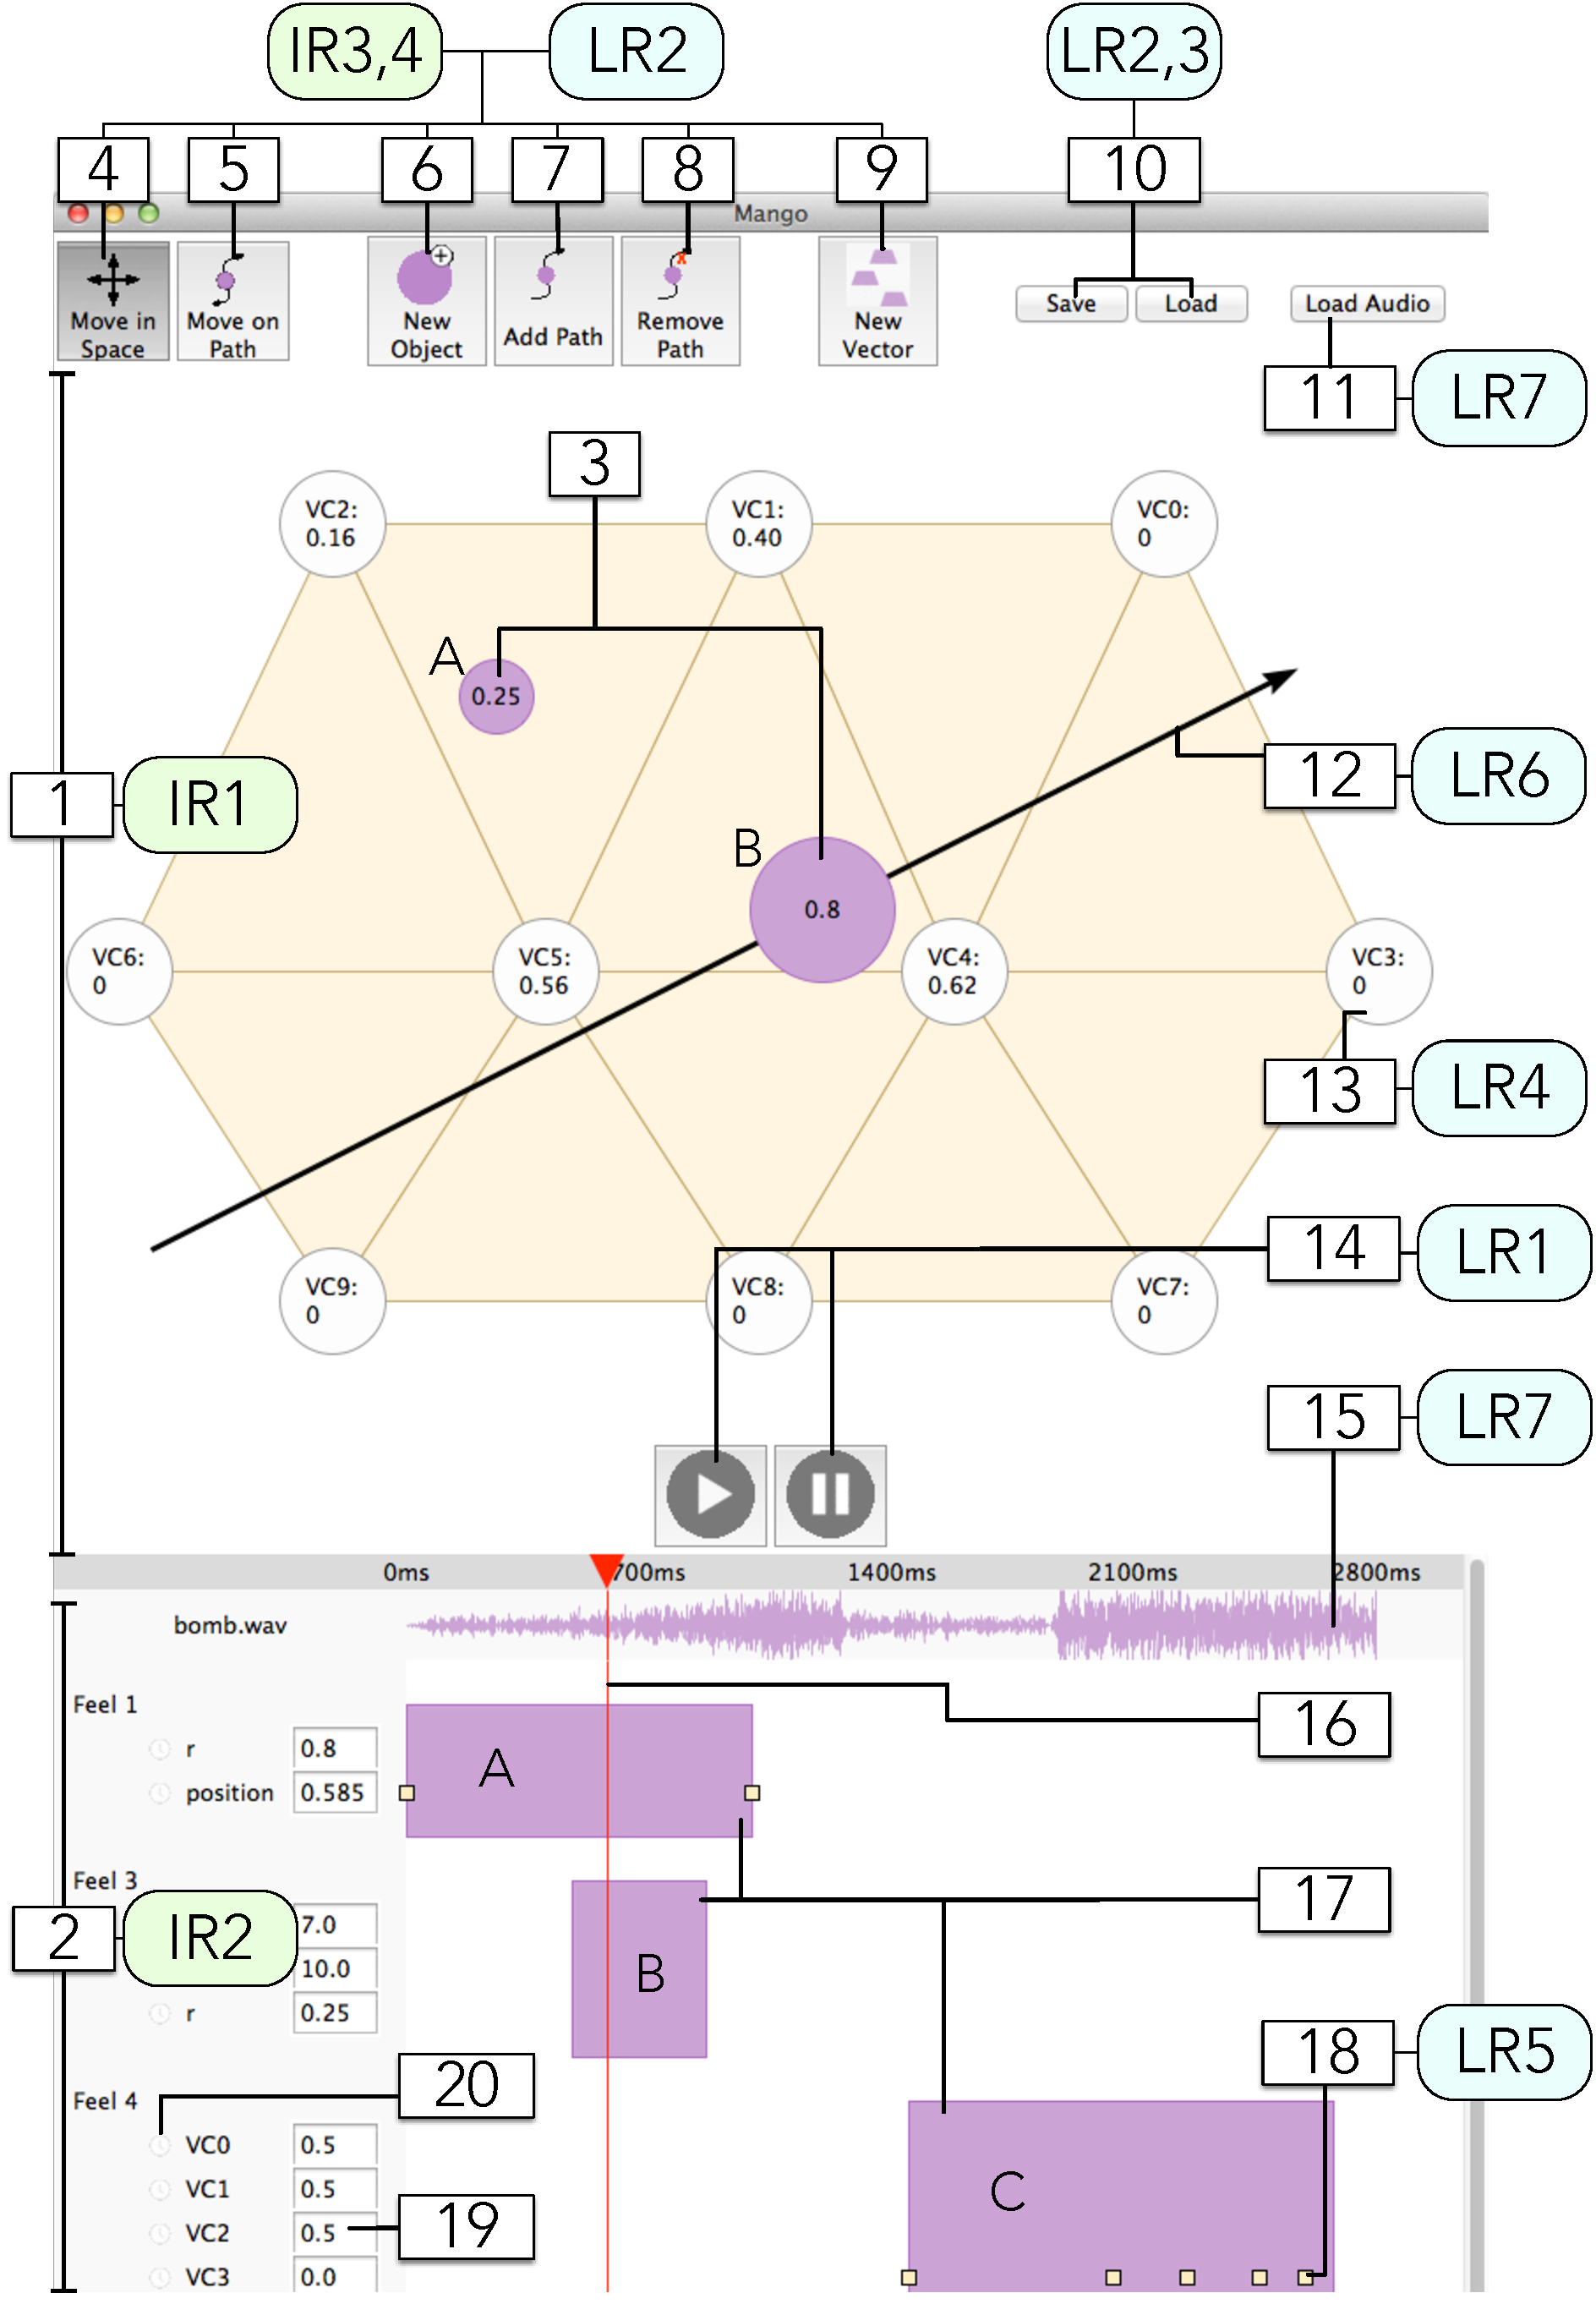
\includegraphics[width=0.77\textwidth]{Mango-Screenshot-Labeled-2015-04-12-1132} 
   \caption{Mango graphical user interface. Key components are labeled and linked to corresponding design requirements.}
   \label{fig:implementation:screenshot}
\end{figure}

% The rendering scheme computes output waveforms for each hardware actuator channel. % of the hardware.
 \begin{figure*}[t] %  figure placement: here, top, bottom, or page
   \centering
   
\includegraphics[width=1.0\textwidth]{images/Fig2-FeelTaxonomy-2015-04-14-1332}%FeelTaxonomy-2014-09-22-0256} 
   \caption{Tactile animation rendering pipeline. Users can: (a) create tactile animation objects; (b) render objects to actuator parameter profiles (such as amplitude) with our rendering algorithm; (c) rasterize vector sensations into frames; (d) play the sensation on the device.}
   \label{fig:feel:taxonomy}
\end{figure*}

\textbf{Vector formats} are similar to those in previous work (e.g., \cite{Enriquez2003}).
Instead of objected-based definitions, as in tactile animation objects, parameters are defined for individual actuation. % in the vector format 
(\autoref{fig:feel:taxonomy}b).
Parameters include duration, amplitude envelopes (e.g., fade-ins and fade-outs), frequency, and start times.
Being device-specific, vector formats % are device-specific and 
offer finer sensation control than tactile animation objects (analogous to pixel-level editing of sprites).
However, creating a single percept from independent controls can be challenging.
This data type is useful when rendering methods for the hardware are not defined or the user wants to control specific actuator sequence to animate tactile content, such as using the Tactile Brush \cite{Israr2011a}. 

\textbf{Raster format}, analogous to a raster-graphics image or WAV file, is suitable for playback operations or exporting it to a device specific format (\autoref{fig:feel:taxonomy}c).
A raster format contains a matrix of actuator intensities; each row defines intensities of an actuator and columns containing the intensities at each time instance. Each format also contains a timestamp row defined by the rendering engine's framerate.  
The playback system parses the raster data, finds the current column, and pushes these actuator settings to the device. %, setting each actuator to its desired value.
This data type is also used for real-time feedback during authoring.
% KM: surely other ways of doing this too.

%In our implementation, all data types are stored as JavaScript Object Notation (JSON) files.
%In the following, we describe features of an authoring interface for designers to create animation sequence; and the empirically determined, high-definition VT rendering method. % for high definition sensations on the VT hardware.


%%%%%%%%%%%%%%
%
% Section - Design
%
%%%%%%%%%%%%%%
\subsection{Authoring Interface}
%%\ALIc we need a good introductory sentense for this section.
The authoring interface % is the key component in the Mango tool and % KM: so is the rendering pipeline isn't it?
allows designers to efficiently create moving tactile content in a familiar environment.
Here we describe user interactions, %to generate animated tactile content, %and associate them with our gathered design requirements. 
% gathered in Section 3. 
% In Mango's implementation, 
most of which
%Most Mango interactions 
are through the animation window (1) and  timeline (2) (\autoref{fig:implementation:screenshot}).
%

%% ------
%\subsubsection{Animation Window and Object Paths}
\emph{Animation Window}: A user creates a tactile animation object (3) with a ``new object" button (6), then manipulates it in the animation window (1). %, which shows its size and position at current time.
The window is overlaid with a faint trace of the % light impression of 
VT hardware (13) for %to give % the designer 
 % so the user can place the object at the right location corresponding to
context. % on the skin. % in contact with the hardware.
%The device configuration file, loaded on startup, provides location and type of actuators, available rendering schemes, and any hardware specific information. 
Here, we used an array of 10 VT actuators (\autoref{fig:rendering}).
%The hardware then generates VT sensations corresponding to animation objects (3). %, in real time, using a rendering algorithm describe in the next section.


\emph{Object Paths}: The animation object (3A) has (x, y) parameters describing position, an ``r" (radius) parameter, corresponding to the VT output voltage from 0 (minimum) to 1 (maximum).
% that is
%scaled to the size of the circle on (1). 
An optional path can be added to an object (7), or removed (8), along which the motion of the object (3B) is constrained (12). 
%Thus, 
The path-object (3B) %has a single ``position" parameter from 0 to 1, instead of (x, y) parameters, and
is manipulated in two ways: moving on path (5), which moves the object from the beginning (position=0) to the end of the path (position=1), or moving in space (4), which moves the object and the path together on the animation window (1).
%The path can be redefined by clicking and dragging boxes at each end of the path.
The current Mango implementation only supports straight-line paths, however their use can be extended in a later version.
Also note that curves can be accomplished through keyframed (x, y) positions.
%Each animation object has at most one path, and each path has only one animation object.
%An alternative model is independent paths, similar to masks in Photoshop or After Effects.
%However, we felt this was too detailed for an early prototype and could confuse users. 

%% ------
%\subsubsection{Timeline}
\emph{Timeline}:  Each animation object (3) is represented in the timeline (2) as a track (17). 
The red scrubhead (16) (shown as a triangle and line) shows and manipulates the current time.
%, and can be dragged around (``scrubbed"). 
Animation objects can be moved in time by clicking and dragging, and resized to change duration. %to have a shorter or longer duration.
Individual parameters can be set on the left, by typing values into text fields (19), allowing precision.
The entire animation can be played and paused using buttons (14) or the spacebar.

\emph{Keyframes}: Parameters can be toggled as ``keyframeable" with a small clock button (20).
%A keyframeable parameter has a value that depends on the current time.
When the value is changed, a keyframe (18) is automatically created at the current time.
Intermediate values are linearly interpolated. %..between. % keyframe values.

\emph{Vector Sensations}:  
% vector sensations for an object (3) can be created by clicking on a button (9) while (3) is selected.
A new vector can be created by selecting an object (3) then clicking on a button (9).
These sensations control each actuator directly through the parameter values, controlling that actuator's voltage from 0 to 1 (same as the ``r" parameter).
%and converts object tracks to individual actuator tracks (17C) in the timeline (2).
The corresponding actuator is highlighted in the animation window (1) when the text field (19) or track (17C) is selected.
Each track is also keyframeable.
%This feature is useful when users need to fine-tune % for users to manipulate 
%individual actuators, and % for fine tuning, as well as 
%to support previous multi-track designs (e.g., \cite{Enriquez2003}).
% and to export time-series waveform to a file (such as a .wav file)

%% ------
%\subsubsection{Save and Load}
\emph{Save and Load}: 
Animations can be saved and loaded (10) to/from JSON files.
% using the data model previously described.
An audio track can be loaded (11) to the timeline (15).% for context (LR7).
This allows the user to design a VT experience for sound files (LR7).
Video overlay is left for future work.% of Mango.

\emph{Hardware Configuration File}:  A hardware-specific structure is defined and stored in a JSON configuration file (LR4). The file contains:
%\kmC{slc} % KM: consider naming these (a), (b) etc to avoid confusion with numbered items in Fig 3
(a) physical width and height of the grid, %in physical units;
%If a hardware has two % separate 
%grids, e.g., on seat and back of %such as one on the seat and one for the back for a 
%chair-like hardware, then individual grid size is defined separated by an identifier.
(b) a dictionary of actuator types (e.g., voice coils or rumble motors), each with a list of control parameters (e.g., frequency, intensity) and allowable values;
(c) location and type of each actuator;
(d) supported communication protocols and rendering methods;
(e) brand information (e.g., USB vendor id and product id) for device recognition; and
(f) default settings.
Physical dimensions are defined in SI units, e.g., meters, Hz. 

\emph{Playback}: Once the animation of the object is defined,
%in both the animation window (1) and the timeline (2),
the user can play and stop the animation. % using buttons (14).
During playback, the animation runs in (1) and the corresponding parameters vary in (2).  
Simultaneously, VT stimulations are activated on the hardware for user feedback.
%and the user feels sensations on the body.  
Multiple animation objects and vector sensations can exist simultaneously.
%, and multiple objects can be grouped together as one object.
Actuators output the sum of all the values generated by objects (described later in the Rendering Algorithm section) and vector sensations.

%Using Mango's user interface, users are able to manipulate animation objects continuously in space and time and vector sensations, which emulates previous tools (e.g., \cite{Enriquez2003}).

    
    
    
%%%%%%%%%%%%%%
%
% Rendering Pipeline
%
%%%%%%%%%%%%%%
\section{Rendering Algorithm}
Mango's rendering algorithm defines how high-resolution haptic feedback is translated to % rendered on
 sparse grids of VT actuators. 
% the central component of the Mango animation tool.
% It makes use of a
The rendering algorithm translates animations created in the animation window to animated VT patterns on the hardware.
\autoref{fig:feel:taxonomy} shows the rendering pipeline that converts animation objects to
%vector sensations and
a raster format, which outputs to the hardware.

The rendering algorithm is derived from %deep and extensive \kmC{SLC} % KM 04.12: are you sure about "deep/extensive"? sounds funny to me.
psychophysical understanding of VT illusions on the skin and creates percepts of virtual actuators and their motion in between a set of real actuators.
The precise perceptual model depends on several factors, such as type of VT actuators (DC vs. voice coil motors), stimulation site (forearm vs. back) and the spacing of actuators in the array (e.g., \cite{Israr2011a}).
To allow for custom framerates and real-time feedback, we generalize from the 1D case (in between two VT actuator along a line) to the 2D case (in between three or more actuators, previously accomplished with non-VT sensations \cite{Tanie1980}).
Thorough investigation of the psychophysical model is beyond our present scope, however, we empirically determine 
the most effective model among those  % optimal model that is derived from various methods
 documented in the literature for the 1D case with a 
% The only 2D phantom sensation of which we are aware was done with electrocutaneous stimulation, not vibrotactile \cite{Tanie1980}.
 %\kmC{2D vs 1D, slc} % KM: don't you need to go into more detail on 2D vs 1D? this seems like it's hinting at something without saying it.
%In this section, we present a renderin algorithm and propose rendering models for 2D actuator grids, extended from prior 1D approaches \cite{Israr2011a,Lee2012a}.
%The rendering algorithm computes output values for all actuators and uses real actuators to create virtual patterns, 
%and requires knowledge of % therefore, the
% location and type of actuators in the hardware. % is an important input. 
%This kind of device abstraction is accomplished through Mango's device configuration file (LR4), whose parameters accommodate a wide range of haptic and VT hardware.
% This and similar hardware-specific information is defined in the device configuration file (LR4) and is uploaded in Mango to accommodate a wide range of haptic and VT hardware in Mango platform.
%Here we describe the interpolation models for rendering algorithm used in the prior literature, and a 
pairwise comparison.
% for the Mango's rendering algorithm.

%\subsection{\kmE{Psychophysics-driven Selection of} Interpolation Models} 
\subsection{Perceptual Selection of Interpolation Models}
The rendering algorithm translates virtual percepts to a physical actuator grid.
We first construct a Delaunay triangulation for all actuators to automatically define a mesh on the hardware grid.
At each instant of rendering, we use barycentric coordinates of the virtual animation objects relative to a triangle defined by three real actuators (\autoref{fig:rendering:algorithm:barycentric}).
Barycentric coordinates are scaled by an interpolation method to determine real actuator intensity.
%These barycentric coordinates scale the intensity of real actuators using interpolation models shown in \autoref{fig:rendering:algorithm:interpolation}.

We propose three interpolation models for Mango, derived from prior psychophysical understanding of phantom VT sensations:
% They are: 
(i) {\it linear}, 
(ii) {\it logarithmic (``log")}, and 
(iii) {\it Pacinian power (``power")} (\autoref{fig:rendering:algorithm:interpolation}). 

In the linear interpolation model, barycentric coordinates are linearly related to actuation amplitude. In the log model, these coordinates are scaled logarithmically, as perceived intensity is related to physical vibration amplitude % in a logarithmic fashion, based on % This model is derived from the fact that the perceived intensity is logarithmic related to the physical amplitude of vibrations 
\cite{verrillo1992perception}. In the power model,  coordinates are coupled to the power (square of the amplitude) of vibrating stimulations \cite{verrillo1992perception}. 
Linear and log interpolation models have been used in the past to express either location or intensity respectively (but not both) of virtual sensations between two vibrators \cite{Seo2013,Alles1970}. A Pacinian power model was used in \cite{Israr2011a} to account for both location and intensity of virtual sensation between two vibrators.

%%  R.T. Verrillo and G. A. Gescheider, "Perception via the sense of touch," in Tactile Aids for the Hearing Impaired, Practical Aspects of Audiology, I. R. Summers, Ed. London: Whurr Publishers, 1992, pp. 1�36. 

%In the following user study, we compare the three interpolation models to determine the best method for our VT hardware. 
%However, a thorough and extensive psychophysical study is left for future work.


\begin{figure}[t] %  figure placement: here, top, bottom, or page
   \centering
  \begin{subfigure}[b]{0.4\textwidth}
	   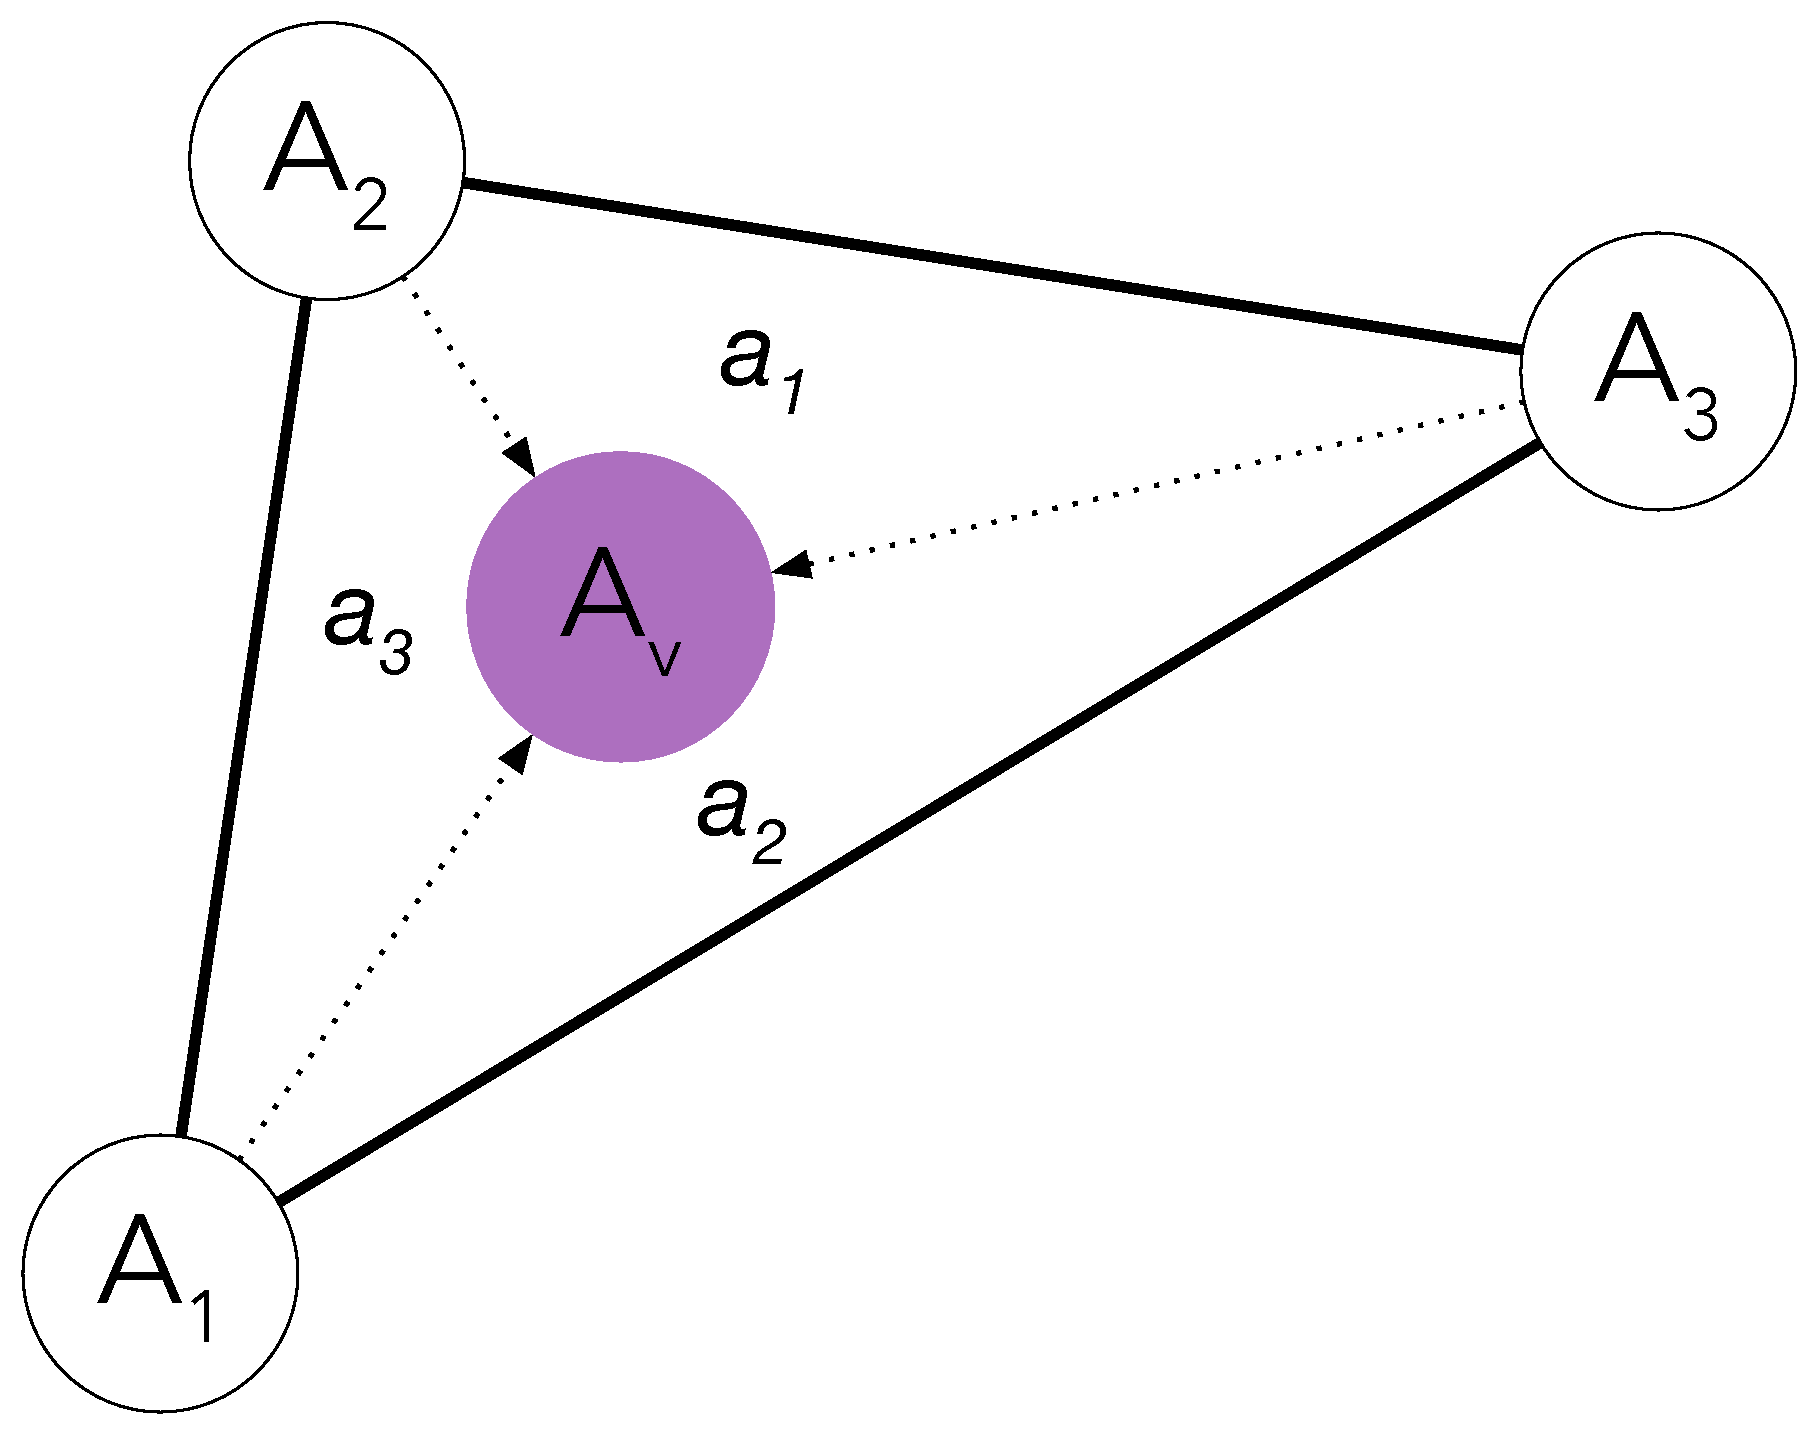
\includegraphics[width=\textwidth]{HA14-RenderingFigure-2015-08-06-1707} 
	   \caption{Barycentric coordinates}
	   \label{fig:rendering:algorithm:barycentric}
    \end{subfigure}
    \qquad
     \begin{subfigure}[b]{0.45\textwidth}
     		\begin{tabular}{l l}
	   	Linear & $A_i = a_i \times A_v$  \\ 
		\\
	   	Log & $A_i = \frac{\log{a_i+1}}{\log{A_{max} +1}}A_v$  \\
		\\
	   	Power & $A_i = \sqrt{a_i} \times A_v$
		\\
		\\
		\end{tabular}
	   \caption{Candidate interpolation methods}
	   \label{fig:rendering:algorithm:interpolation}
    \end{subfigure}
    	   \caption{Interpolation models to determine physical actuator output ($A_{1-3}$) from virtual actuator intensity ($A_v$) and barycentric coordinates ($a_{1-3}$).}
	   \label{fig:rendering:algorithm}
\end{figure}



%%%%%%%%%%
%
%
%
\subsection{Pairwise Comparison Study}

% Our first study is 
%We performed a pairwise comparison between the three candidate interpolation models prototyped for Mango's rendering pipeline.
%Our goal was to determine the user-preferred model for this VT hardware, to be used in Mango's ongoing implementation; and to identify relevant factors (e.g., frequency, amplitude, or individual differences).
To determine the preferred model for this VT hardware in Mango's rendering pipeline, and to identify relevant factors (e.g., frequency, amplitude), %, or individual differences), 
we performed a pairwise comparison of our three candidate interpolation models.

\subsubsection{Participants and Apparatus}
Eighteen volunteers took part (6 female, between age 20-35). % aged 21 to 34) . 
%
The VT hardware consisted of 10 high-quality VT actuators (C2 tactors, Engineering Acoustics, Inc., USA) arranged in a 3-4-3 layout and mounted on the back of a chair in a pad  21 cm high, 29 cm wide, and 2 cm thick;  actuators form equilateral triangles with edges of 6.35 cm  (\autoref{fig:rendering:device}). The rendering engine updates at 100 Hz.
Through piloting, we determined that the device's on-screen visual outline should mirror the sensations rendered on the physical device. That is, if participants see an animation object on the right side of the screen, they prefer to feel it on the right side of the back. 
% (as if they are looking from behind the VT hardware). 
\autoref{fig:rendering:study} shows the experiment interface, in which an arrow represents the sensation direction. 


\begin{figure}[t] %  figure placement: here, top, bottom, or page
   \centering
   \begin{subfigure}[b]{0.37\textwidth}
	   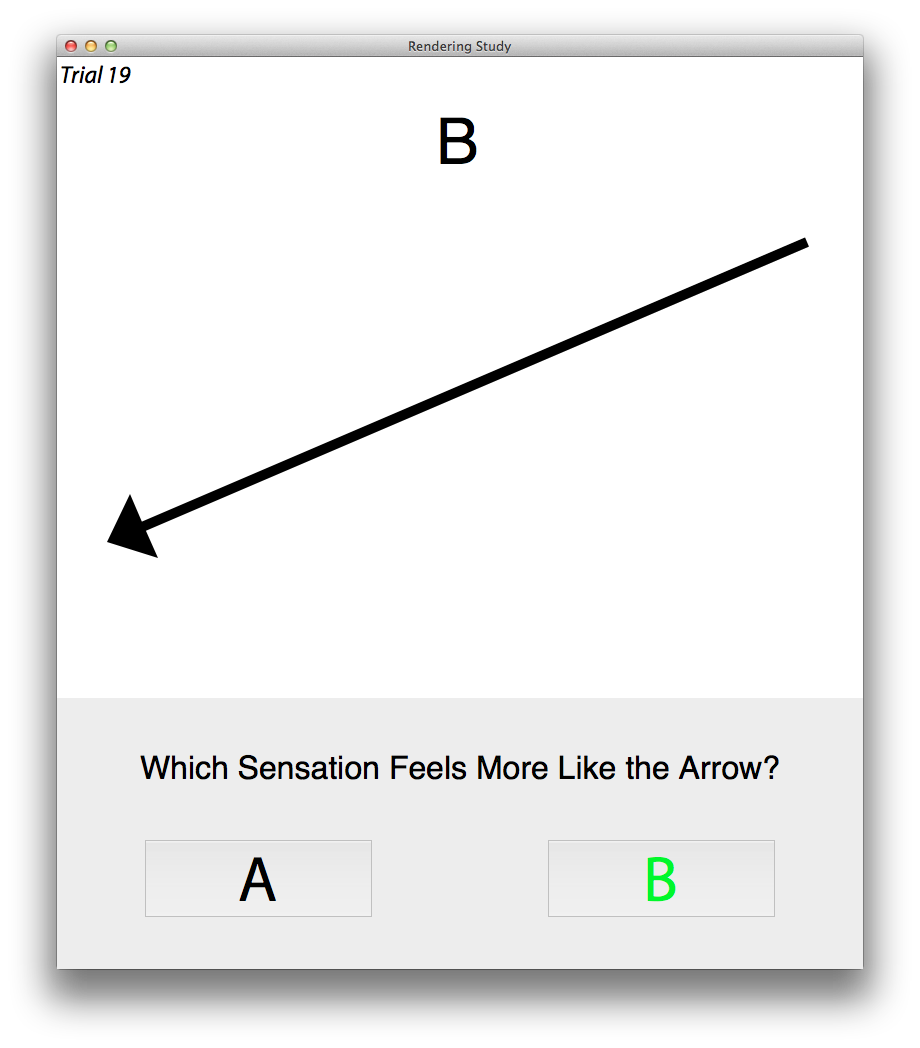
\includegraphics[width=\textwidth]{HA14-RenderingUI-2014-08-19-1417} 
	   \caption{Rendering study interface}
	   \label{fig:rendering:study}
    \end{subfigure}
    \qquad
     \begin{subfigure}[b]{0.55\textwidth}
	   	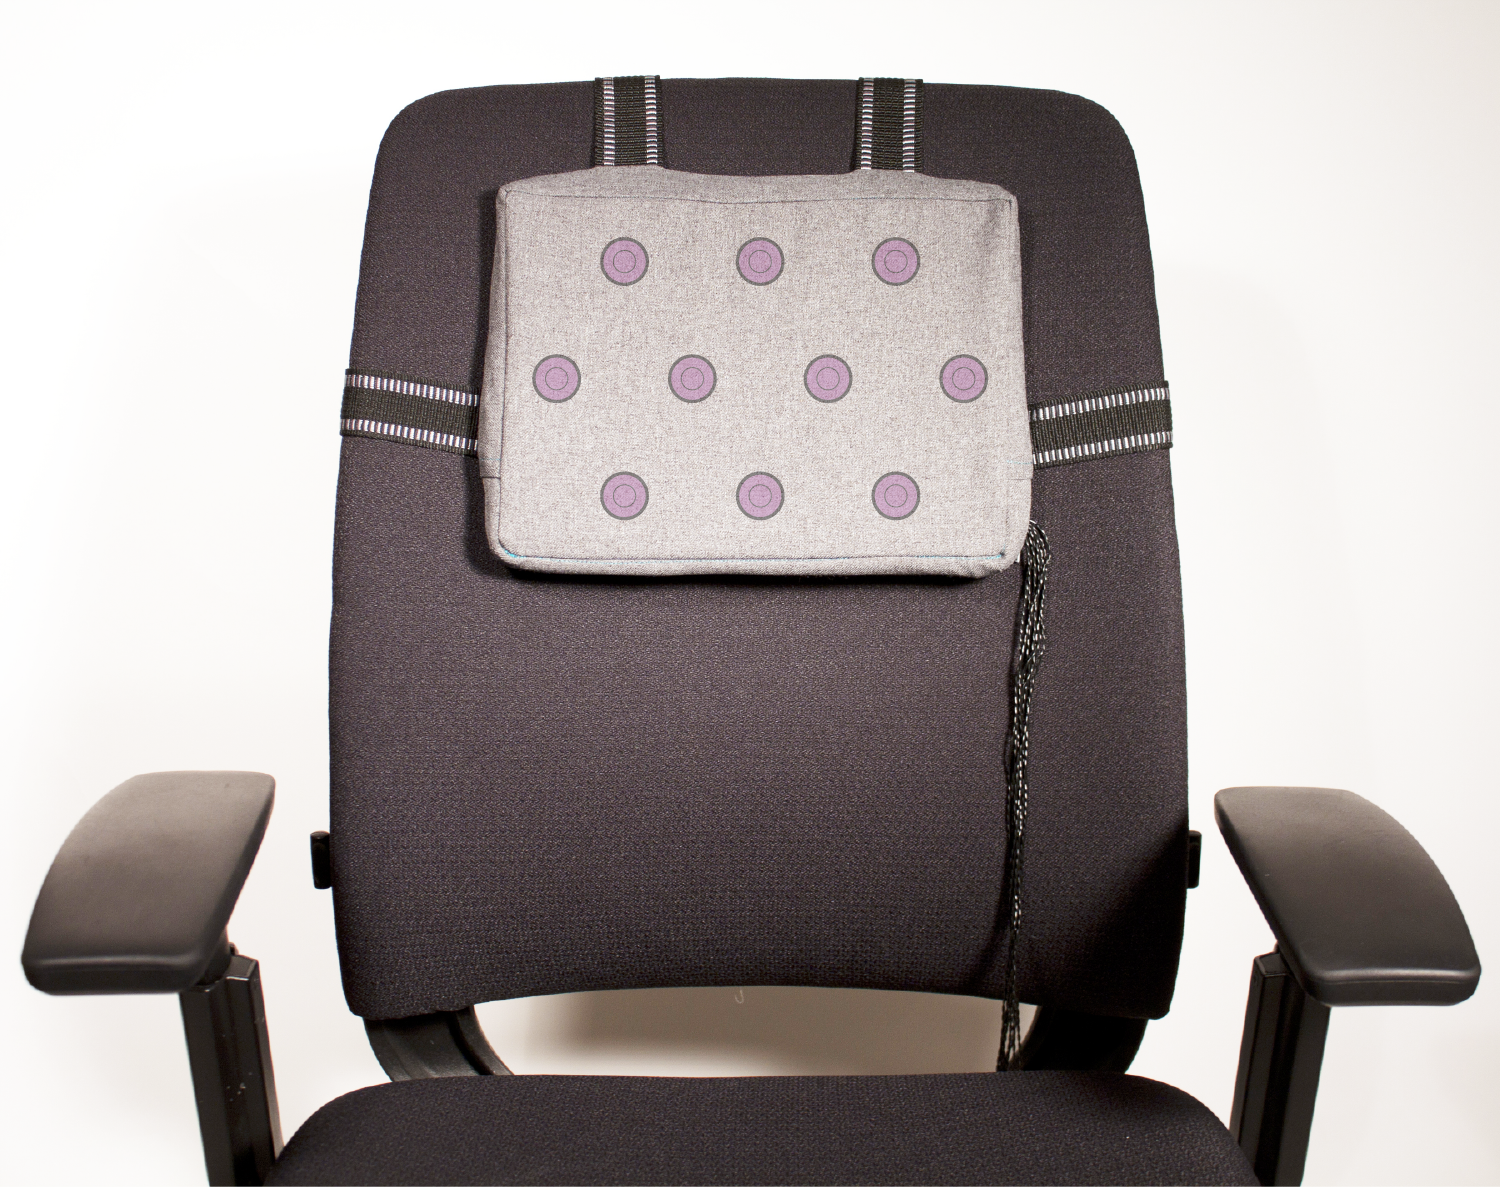
\includegraphics[width=\textwidth]{figure_chairpad} 
	   \caption{Output device with highlighted actuators}
	   \label{fig:rendering:device}
    \end{subfigure}
    	   \caption{Rendering study setup and user interface.}
	   \label{fig:rendering}
\end{figure}

\subsubsection{Methods}
We conducted % a series of 
A/B paired comparison tests (two-alternative, forced-choice) to determine the preferred model out of the three candidates.
%
In each trial, participants were presented with two stimuli at % separated by 
a 400 ms interval.
Each stimulus is
%a rendition of
a ``straight-line" VT stimulation on the back using one model. % of the three interpolation models.
%Stimulus frequency, intensity, direction, and duration were constant across trials. \kmC{slc} % KM 04.12: what is 'across trials'? next para, you refer to these as controlled variables, so I'm a little confused.
Participants were asked to % compare the two stimuli and 
select the stimuli that \emph{best represented straight-line motion} in a variety of directions.

Two durations (500 and 1500 ms), eight cardinal directions, and A/B order were crossed with each model pair, and presented in a random order.
For each trial, frequency was randomly selected from 80, 160, 240, and 300 Hz, and intensity from between 10 and 20 dB above detection threshold.
Each participant performed 96 trials over $\sim$15min (1728 total). 

\subsubsection{Results}
% Analysis was conducted for each pairwise algorithm matchups. % We fit the data
Each algorithm pair's data was fit  to a logistic regression model with participant, frequency, intensity, direction, and duration as factors;  direction was grouped into horizontal, vertical, and diagonal.
We performed stepwise regression (backwards elimination with $\alpha=0.05$ and a $\chi^2$ test for removing each factor) to iteratively eliminate factors that were not statistically significant. % , then analyzed the result.

\emph{Logarithmic vs. Linear.}
% We 
Regression eliminated % 4 factors: 
duration, frequency, intensity, and direction ($p>0.1$).
The resulting model has Nagelkerke $R^2=0.135$.
Using Bonferroni correction for multiple comparisons, 95\% confidence intervals for each participant were computed. 
11 participants were more likely to prefer Log over Linear ($p<0.05$) models; none were likely to prefer the Linear model.

\emph{Logarithmic vs. Pacinian power.}
All 5 factors were eliminated ($p>0.1$).
The overall 95\% confidence interval of participants selecting Log over Power was 37.06\% to 87.40\%, overlapping 50\%.
We therefore detected no significant difference of preference between Log and Power models.

\emph{Pacinian Power vs. Linear.}
We eliminated %3 factors:
intensity, direction and duration ($p>0.1$), with the fitted model's %The fitted model had 
Nagelkerke $R^2=0.0970$.
The confidence interval for each participant-frequency combination, via Bonferroni corrections, yielded 22 / 72 participant-frequency combinations selecting Power model over Linear model more than 50\% of the time.
No one chose the Linear model more than 50\% of the time.

\textbf{Conclusion:}
Logarithmic interpolation outperformed linear and was % found 
equivalent to Pacinian power model. We proceeded with the logarithmic model for Mango's implementation, as the power model did not outperform either of the others. % the linear model.
%\kmC{ based on its greater simplicity of implementation. ???}
% Of the three candidate algorithms, we chose the Logarithmic interpolation method for the rendering algorithm of the Mango animation tool. 

%%%%%%%%%%
%
% Animation Tool Evaluation
%
\section{Design Evaluation}
% We implemented the critical functional features of Mango as described in the above sections.
To evaluate Mango's % the 
animation metaphor and expressive capability,
%with critical functional features implemented,
we asked media professionals to
% we had media professionals 
create a variety of designs.
Qualitative evaluation was chosen for rich, focused, early feedback of the animation metaphor and lessons for iteration.
A quantitative comparison between tool perspectives is left until more refined tools are developed.
We wanted to establish whether this is an effective approach before studying the most effective approach.


Six participants (P1-6, 3 females) were introduced to Mango driving % linked to 
the  VT hardware described previously. % for the pairwise comparisons. 
%First, each participant was interviewed about their background.
P1 had experience with haptics but not animation beyond video editing;
P2-5 had animation experience but little or no experience with haptics;
P6 had no experience with haptics or animation, but was familiar with media tools like Adobe Photoshop.
P5 was also involved with the requirement gathering interviews presented earlier.
Each entire session took 40 to 60 minutes.


Each participant was introduced to Mango with a training task: % and the use of tactile animation objects and vector sensations.
designing an alerting sensation using %  ``alert" sensation with 
either animation objects or vector sensations (order counterbalanced).
%half of them used the animation objects first and the other half used vector sensations first.
Then, each participant was given three design tasks.
1) Primarily \emph{temporal}: create a heartbeat sensation.
2) Primarily \emph{spatial}: tell a driver to turn left.
3) \emph{Context-based}: create a tactile animation to match a sound file.
A 3-second sound effect of a bomb falling (with a whistle descending in pitch) then exploding with a boom was chosen, i.e., complex with two semantic components.
The wide array of resulting designs can be found in the accompanying video.
Mean non-training task time was 5:59 (med 5:38, sd 2:46, range 1:41-13:48).

After each task, participants rated confidence in their design from 1 (Not confident) to 5 (Very confident), primarily to stimulate discussion.
All designs were rated 3 or higher; P6 wrote ``6" for his sound-based design.
The animation object training task was always rated the same or higher than the corresponding vector training task.
While suggestive, these ratings were self-reported and from a small sample.
We thus did not conduct statistical analysis.
%, due to small sample size.

%
% Show one animation
%
\begin{figure}[htb] %  figure placement: here, top, bottom, or page
   \centering
%   	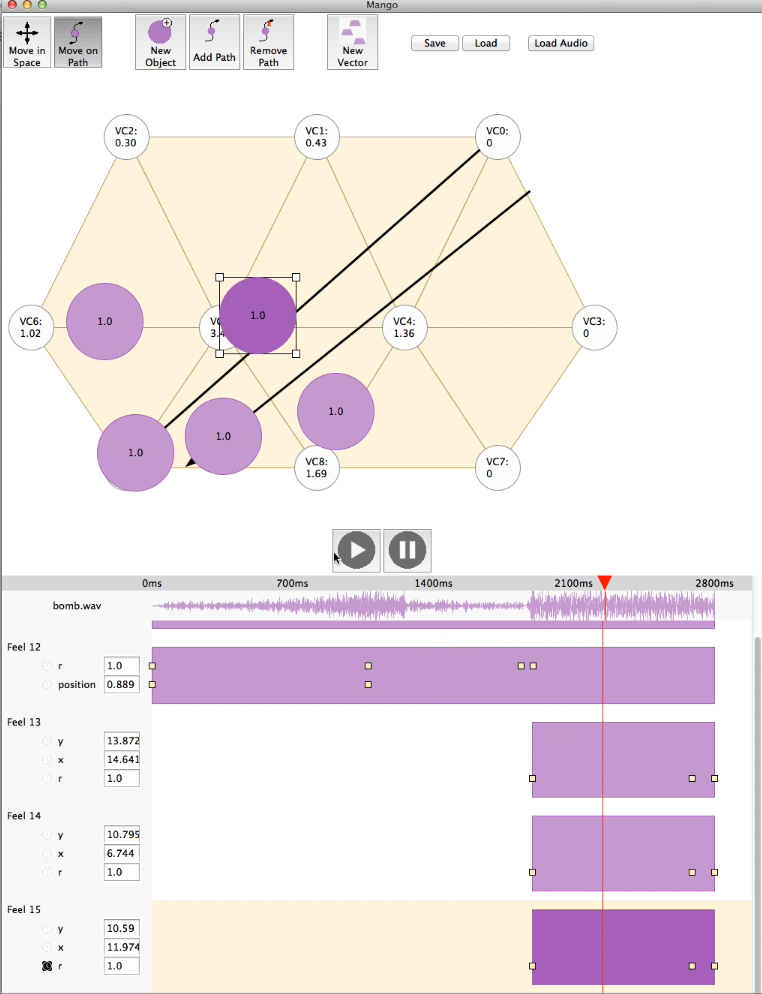
\includegraphics[clip=true, trim= 1 150 0 7, width=0.4\textwidth]{P2_sound_example-2014-09-22-1630} 
	   	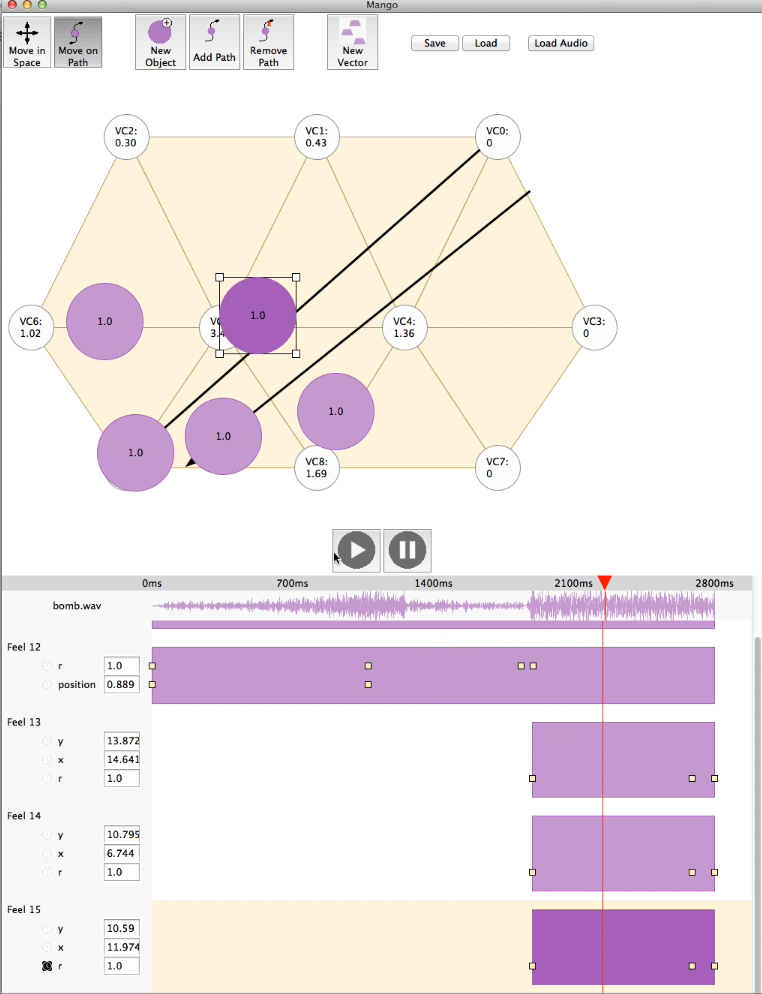
\includegraphics[clip=true, trim= 4 155 0 85, width=0.8\textwidth]{P2_sound_example-2014-09-22-1630} 

	\caption{Example of P2's animation for matching a sound. See the accompanying video for all participant animations.}
	\label{fig:animation:example:p2}
\end{figure}




A semi-structured interview followed the design tasks.
%The interviewer then followed up on interesting statements and/or concerns.
Participants were asked to compare animation objects with vector sensations, and to walk through the interface to elicit feedback.
%
% Study 2 results
%
%\subsection{Results}
Interviews were conducted and analyzed by a researcher with training and experience in qualitative research, and followed established methodologies:
% by considering each statement, memoing, coding, and relating codes
%according to % Corbin and Strauss's 
methods of grounded theory  \cite{Corbin2008} informed by phenomenological protocols \cite{Moustakas1994}.
Analysis resulted in four themes.

\subsubsection{Theme 1: Animation Metaphor}
Participants found the tool easy to use.
All six participants were able to accomplish all five tasks (object alert, vector alert, heartbeat, turn left, sound).
Participants described the interface as intuitive (P1-5), agreeing that it was an animation tool: \qq{It's up to the standards of other animation tools}{P1}, \qq{This is totally animation}{P2}, \qq{It felt very much like an animation tool}{P4}, \qq{I'm not an expert when it comes to haptics, but this software seems almost as if it can change the game of designing haptic vibrations}{P5}.
Negative feedback focused on polish and feature completeness:
% not implementing enough features of their preferred tools and general feedback on polish and streamlining of the interface:
\qq{gotta spline [the keyframe interpolation]}{P2}, \qq{a couple quirks but there was nothing difficult to overcome}{P4}, \qq{being able to design your own curve [path] would be really nice}{P5}.
%, \qq{move in space and move on path can be one thing}{P6}.


\subsubsection{Theme 2: Tactile Animation Object vs. Vector Sensations}
Participants relied more on animation objects %  used animation objects more frequently
than vector sensations, which
%Vector sensations 
were only used twice: P4's heartbeat task and P5's sound task (combined with an animation object).
P1 switched from vectors to animation objects early in her heartbeat task;
%for her remaining tasks
no other participants used vector sensations.


Animation objects were described as easier to use and more intuitive, especially to represent location or for non-animators. \qq{After using the new object I'd probably never use new vector again}{P2}, 
%especially to describe motion or position:
\qq{easier to find the location of the heart}{P1}, 
%They were also described as more appropriate for people without animation experience:
\qq{if I weren't an animator I think I would only use [animation objects]}{P4}.
%, \qq{You have to be a little more careful when animating [vector sensations]}{P5}.
%
%Animation objects and vector sensations supported different workflows. Animation objects tended to be described as better for position, movement, and for % if you wanted to have 
%multiple objects, while 
Vectors were preferred for more fine-tuned control when motion didn't matter as much, often using many keyframes.
\qq{You can control multiple [actuators] at the same time, so you don't have to create new objects and then put them everywhere on the screen}{P1},
\qq{[Animation objects] can be more comfortable to use when one doesn't work with keyframes}{P3}, 
\qq{If you want precise control over [actuators], then vector is the way to go}{P4}.
%Participants rarely combined the two:
%\qq{I'm already into the object mode, I forget about the vector}{P6}.

%
% Shows three animations
%
%\begin{figure*}[htbp] %  figure placement: here, top, bottom, or page
%   \centering
%      	\begin{subfigure}[b]{0.30\textwidth}
%		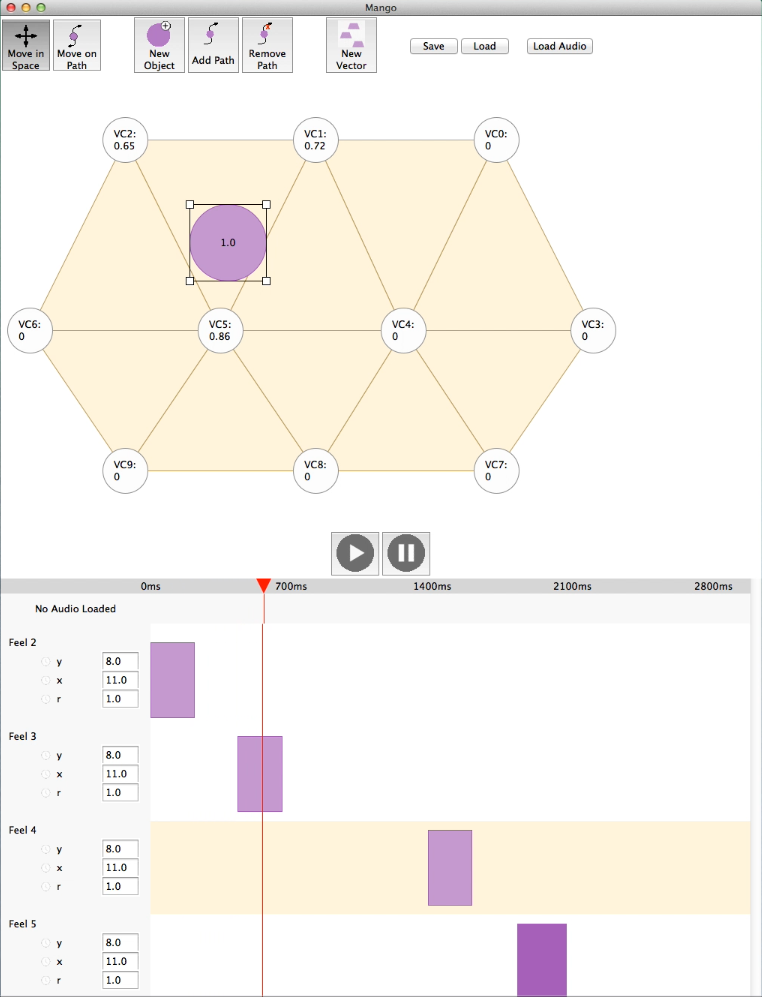
\includegraphics[width=\textwidth]{p1-heartbeat-example} 
%		\caption{Heartbeat task by P1}
%		\label{fig:animation:example:p1}
%	\end{subfigure}
%	\quad
%	\begin{subfigure}[b]{0.30\textwidth}
%		   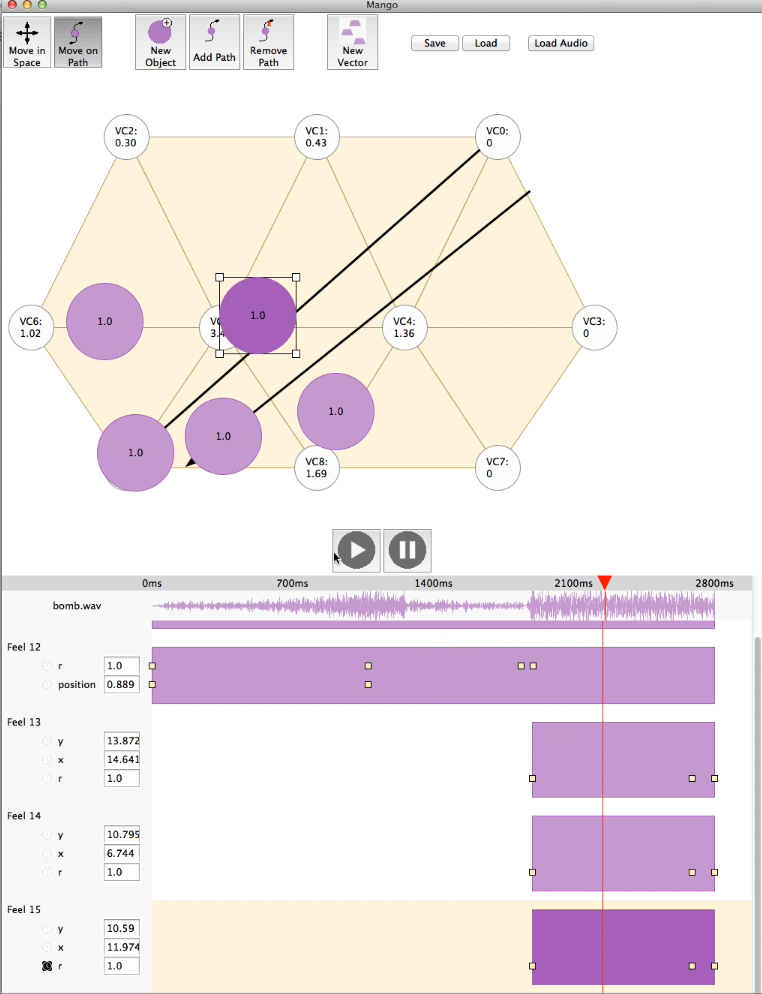
\includegraphics[width=\textwidth]{P2_sound_example-2014-09-22-1630} 
%		   \caption{Sound task by P2}
%		   \label{fig:animation:example:p2}
%	\end{subfigure}
%	\quad
%	\begin{subfigure}[b]{0.30\textwidth}
%		   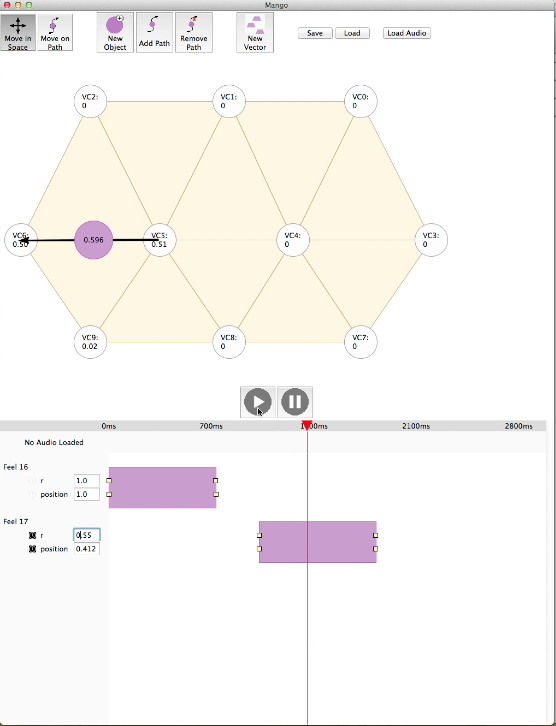
\includegraphics[width=\textwidth]{p4-turnleft-example-2015-01-19-1024} 
%		   \caption{Turn left task by P4}
%		   \label{fig:animation:example:p4}
%	\end{subfigure}
%
%
%
%
%      	\caption{Examples of Animations}
%	\label{fig:animation:example}
%\end{figure*}


%\theme{4}{Feedback, Context and Imitation}
\subsubsection{Theme 3: Designing-in-action with direct manipulation}
Participants used direct manipulation to feel their designs in real time, %  was valuable to participants.
dragging animation objects %in the animation window
and scrubbing through
%at various speeds in
the timeline: \qq{I would make the [animation] object and just play around with it before creating the animation, as a way to pre-visualize what I was going to do}{P5},
\qq{I kind of play around with it, and randomly come up with the ideas}{P6}.
P2 even noted that YouTube did not have
 real-time video scrubbing feedback like Mango's:
 %support for haptic and audio feedback:
 \qq{I wish I could scrub back and forth [with YouTube]}{P2}.
However, continual % constant 
vibrations were annoying, and participants requested a ``mute" feature:
%A VT feedback ``mute'' would be welcomed.
%P4 and P5 moved the timeline so that no output would play during design phase. 
% was playing while they were in design phase.
%\qq{It would be nice if when I [enter values into text fields] it doesn't go off constantly, it's getting annoying}{P3}.
\qq{It would be nice if...it doesn't go off constantly.}{P3}.
%It was further suggested that each object should be independently mutable (as in hiding Photoshop layers), and VT output should be mutable entirely. 

More generally, participants used feedback from their experience or external examples.
P1 stopped to think about her own heartbeat,  P2 used a YouTube video of a heartbeat as a reference, and P3 based her alert on her phone: %directly stated that she
%used imitation for the non-sound tasks
%;  her alert consisted of two vibrations similar to her phone: 
\qq{It's typical to have two beeps for mobile phones}{P3}.
Correspondingly, participants were excited when prompted by an audio sensation: \qq{I was really happy with the bomb one, because I could really hear it and imagine me watching a TV and then feel it at the same time}{P1},
\qq{The sound part was good, that would be a fun thing to design for}{P4}.



\subsubsection{Theme 4: Replication through Copy and Paste}
Replication in both space and time was common while using Mango.
Many designs had symmetrical paths to reinforce sensations (\autoref{fig:animation:example:p2}).
All but P4 requested copy / paste as a feature.
%, suggesting it would be useful (P2, P3), faster (P1, P2) and easier (P5).
%P1, P2, and P5 wanted to duplicate their heartbeat sensation to be multiple beats, but did not do so without copy and paste.
%, instead saying they would repeat or loop it. [??????]
\qq{I could just copy/paste the exact same thing on the left side and then move it to the right side}{P1}, \qq{I have the timing the way I like it, ideally it'd be cool if I was able to copy and paste these, so it would be able to repeat}{P5}.
%\qq{Is there any way to copy and paste keyframes?}{P2}.

\section{Discussion}
Here we interpret our design evaluation, explore animation with other devices, and describe applications and limitations.

\subsection{Design Evaluation Summary}
From our design evaluation, we conclude that tactile animation is a promising approach for controlling tactile grids.
Direct, continuous manipulation of tactile animation objects supported embodied design and exploration by animators, who rapidly iterated on designs to try new ideas.
Mango facilitated the design of a wide variety of animations (see accompanying video) and received positive responses.
We also found recommendations for our next iteration: more animation features, video as well as audio context, and muting.% (similar to hiding layers in Photoshop).%'s ``hide layer'' functionality).

\begin{figure}[htb] %  figure placement: here, top, bottom, or page
   \centering
   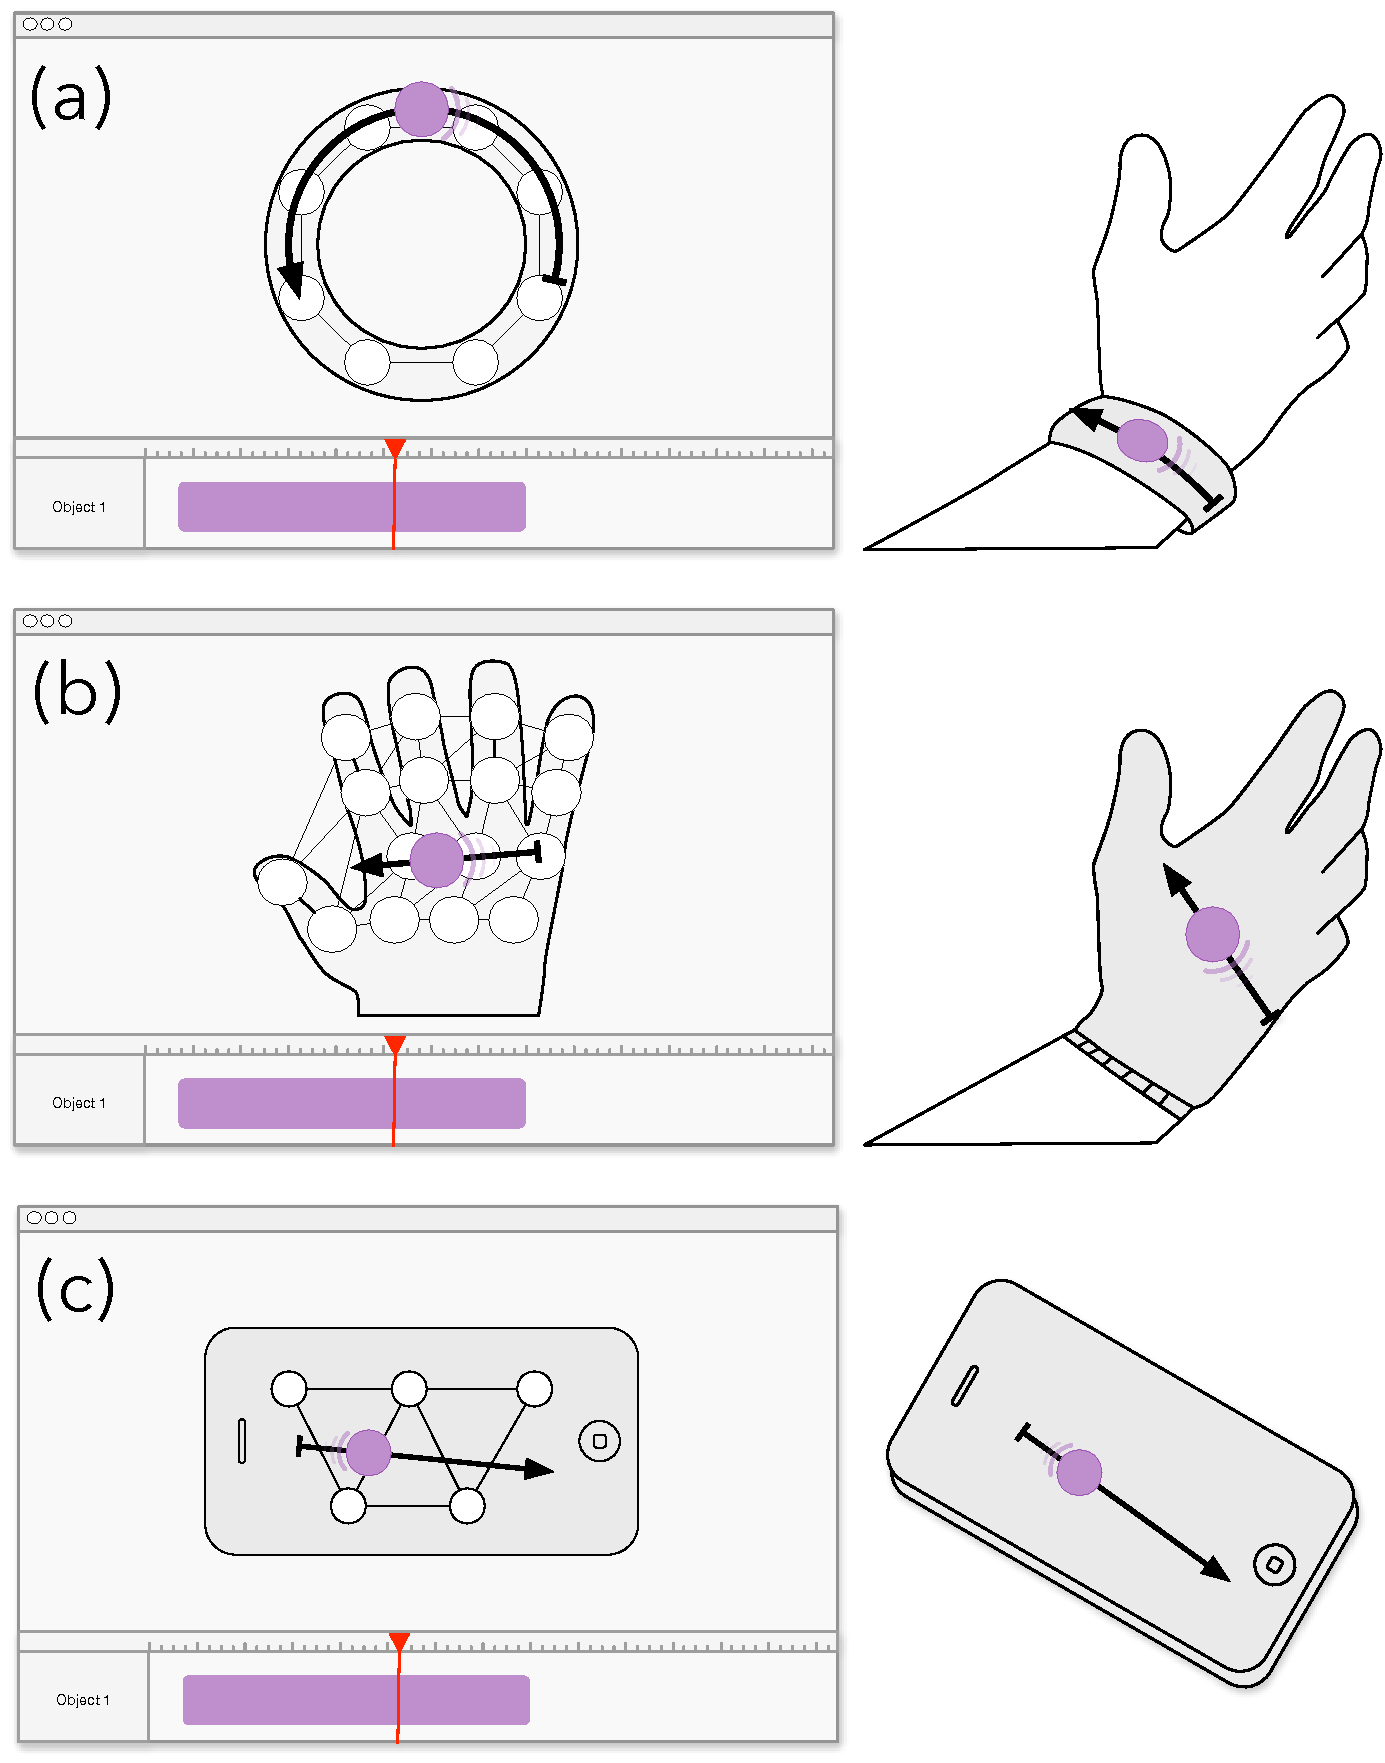
\includegraphics[height=2.75in]{HA14-Applications-Split1-2015-04-14-1025} 
%   \caption{Tactile animation could define motion with (a) 1D actuator arrays, (b) dense and sparse VT grids, (c) handhelds.}
%   \label{fig:application:space}
%\end{figure}
%\begin{figure}[htb] %  figure placement: here, top, bottom, or page
%   \centering
\qquad
   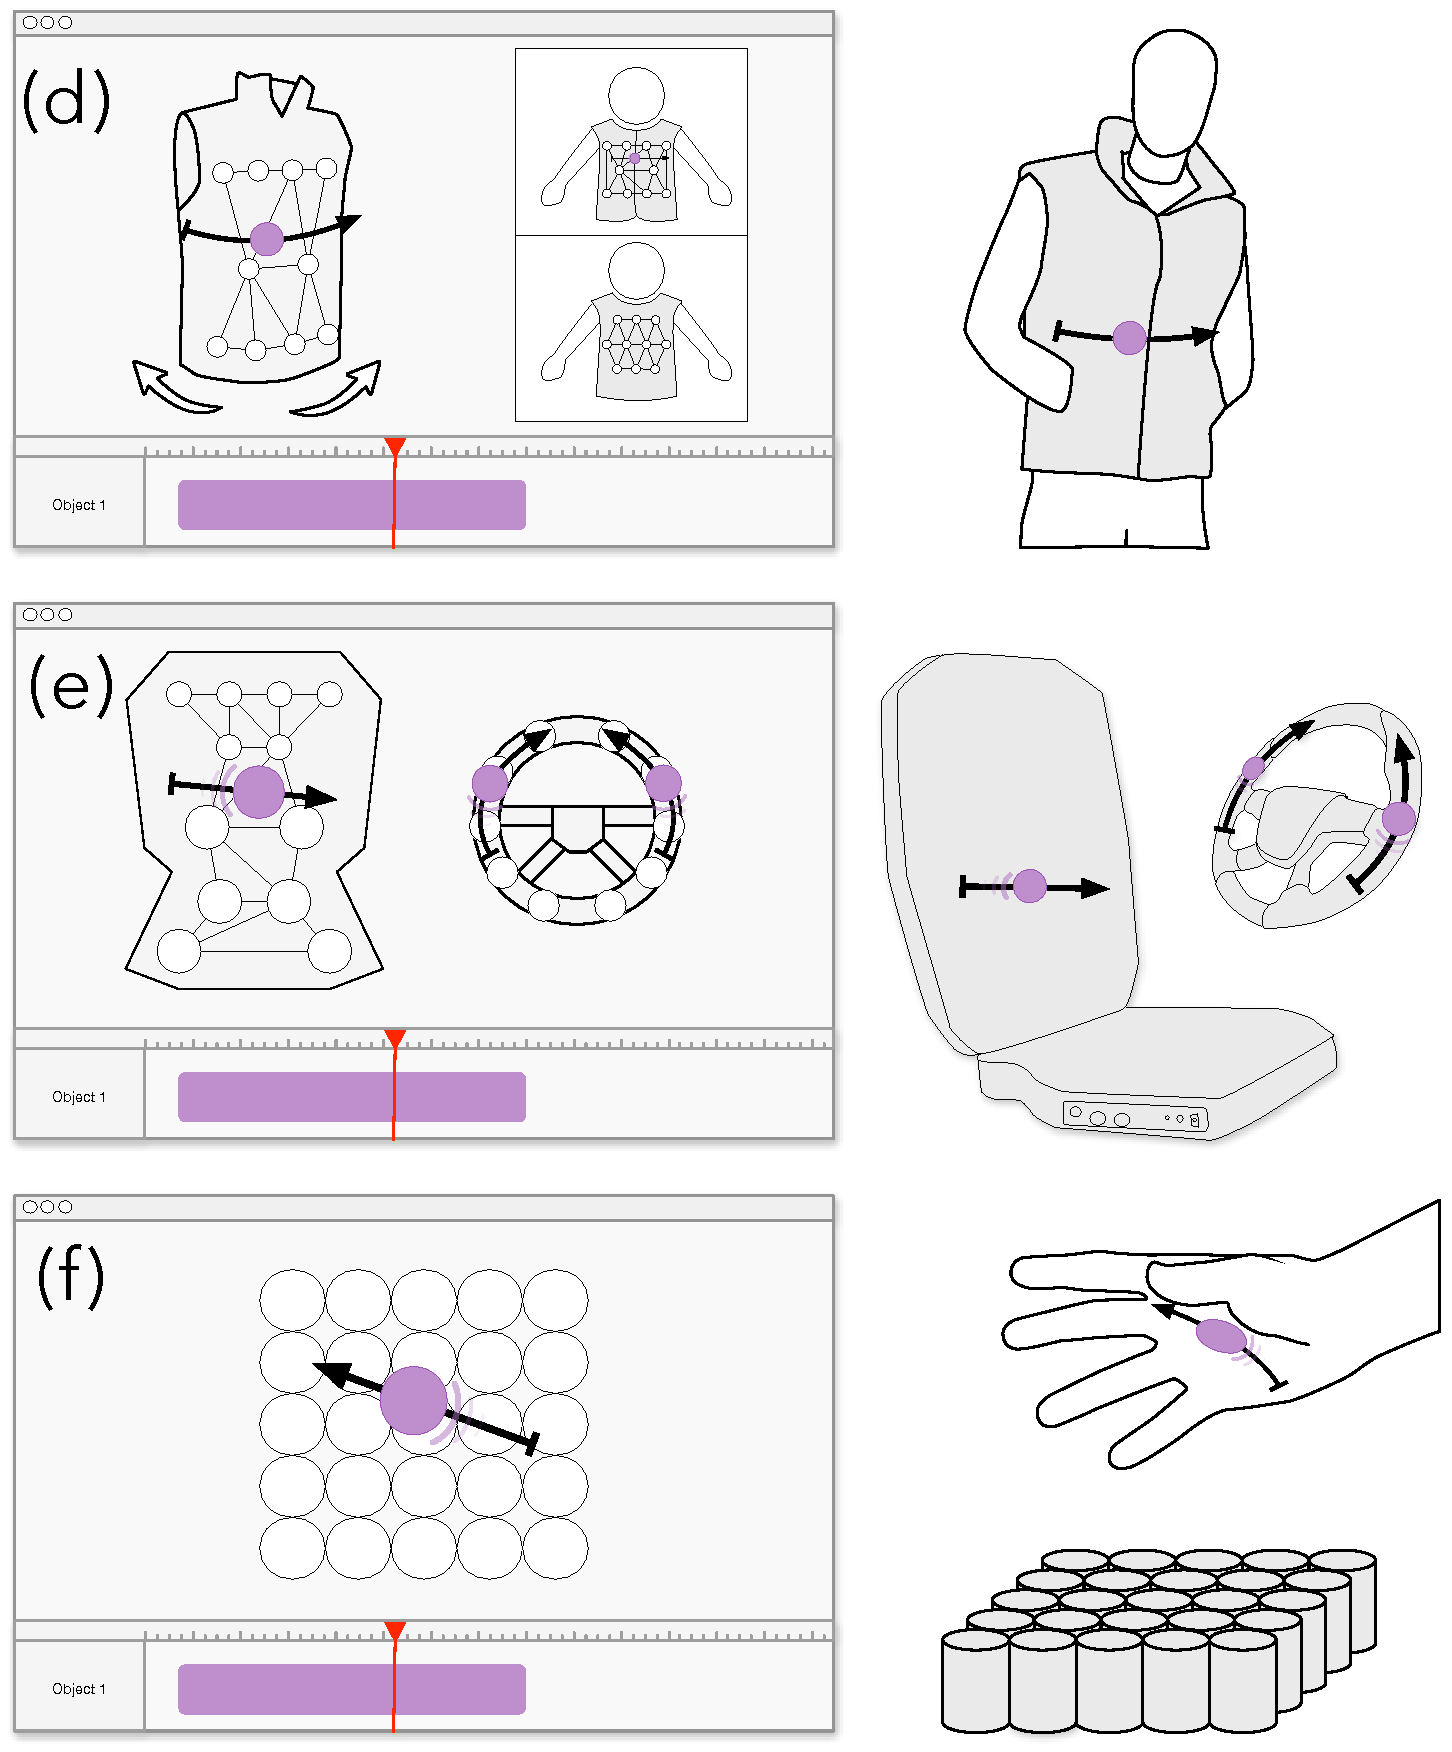
\includegraphics[height=2.75in]{HA14-Applications-Split2-2015-04-14-1025} 
%   \caption{Tactile animation could also define motion  with (d)  3D surfaces, (e) multi-device contexts, and  (f) non-VT devices like mid-air ultrasound.}
%   \label{fig:application:space}
      \caption{Tactile animation could define motion with (a) 1D actuator arrays, (b) dense and sparse VT grids, (c) handhelds, (d)  3D surfaces, (e) multi-device contexts, and  (f) non-VT devices like mid-air ultrasound.}
   \label{fig:application:space}
\end{figure}

%\vspace{20pt}
\subsection{Possible Extension to Other Device Classes}
%\emph{Future Work: Applications and Extensions}\\ % Application space }\\
%We look forward to extending Mango to other devices.
% Mango is not limited to
The animation metaphor is not limited to a back-based pads.
Part of the advantage of an abstracted animation object is that, 
as long as a suitable rendering algorithm can be developed, the metaphor can apply to other devices.
In this section, we illustrate possibilities that we plan to explore in future work.


\emph{1D VT Arrays (\autoref{fig:application:space}a)}:
1D VT arrays are common in arm sleeves, wrist bands, belts, and similar wearables.
These devices provide sensations along the path of the array.
By constraining objects to a linear or circular path, barycentric coordinates collapse into 1D interpolation.

\emph{Dense and Sparse VT Grids  (\autoref{fig:application:space}b)}:
2D VT grids are also common, used in chairs, gloves, and the backs of vests.
%Dense arrays previously had their own actuator-based authoring tools \cite{Kim2009}.
While we evaluated Mango with a sparse back-mounted array, tactile animation naturally supports denser arrays, either with our rendering algorithm or by using a nearest-neighbour technique to activate a single actuator.
%; in both cases, animation objects can be directly manipulated.
%In the present work, we evaluated the usability of Mango to author variety of VT sensations on sparse arrays.
%The actuator layout in both these devices are dif- ferent, and we accomodated them by selecting an appropriate
%algorithm and layout to render high definition haptic feedback.


\emph{Handhelds (\autoref{fig:application:space}c)}:
Actuators embedded in handheld objects, such as mobile devices, game controllers, or steering wheels, shake objects instead of directly stimulating the skin.
Animators might be able to define source locations for vibrations using handheld-based rendering algorithms (e.g., \cite{Seo2013}).
%Similarly, a single embedded vibrator in handheld devices can be supported by constraining the tactile object to a single point.


\emph{3D Surfaces  (\autoref{fig:application:space}d)}:
Mango currently only supports a 2D location for its animation objects.
However, tactile animation can be extended to support surfaces of 3D surfaces, such as vests or jackets that wrap around the user's body. 
More work will need to be done to perfect this interaction style, possibly using multiple views or a rotatable 3D model with animation objects constrained to the surface.
%, drawing more from 3D animation tools like Maya.

\emph{Multi-device contexts  (\autoref{fig:application:space}e)}:
Mango's rendering algorithm already supports connections to multiple devices simultaneously.
The editing interface could combine layouts for different devices, enabling animators to animate the entire user experience (such as a car's seat and steering wheel).

\emph{Non-vibrotactile devices (\autoref{fig:application:space}f)}:
While our rendering algorithm is particular to VT arrays, a tactile animation object can represent manipulable percepts with other actuation technologies.
%Mango is not limited to only VT devices, similar to the one used in the present evaluations.
Ultrasound-based mid-air displays generate a sensation as a focal point with a position and size \cite{Wilson2014}; this sensation could be manipulated through a tool like Mango.
% produce a percept of object in mid-air and can be manipu- lated by changing the focal point as a animated object on the Mango interface. Algorithm to generate localize percept can be loaded along with the specifications written in the config- uration file.
Similarly, passive force-feedback sensations (e.g., Hapseat \cite{Danieau2012a}) or height displays (a grid of pins) could be supported.


%Beyond the VT pad used in our evaluations,
%the animation metaphor naturally supports other devices, some of which have been controlled by other authoring tools (\autoref{fig:application:space}).
%By constraining animation objects to a circular path, wristbands and belts can be supported (\autoref{fig:application:space}a).
%Dense, regular displays, such as glove-based grids \cite{Kim2009}, could also be controlled with direct manipulation (\autoref{fig:application:space}b).
%An extension to vests and other cylindrical or spherical displays might use multiple views to facilitate design (\autoref{fig:application:space}c).
%Finally, complex multi-device scenarios can be coordinated in a single interface (\autoref{fig:application:space}d).
%We have already extended Mango to support a chair-based display (similar to \cite{Israr2011a}), with planned extensions for vests and gloves (\autoref{fig:devices}).

\subsection{Interactive Applications}
While our goal was to enable animators to create rich content, the tactile animation object can be linked to alternative input sources for other interactive experiences.

\emph{User gestures.}
User gestures and motion can be tracked and mapped to animation objects directly rendered on the haptic hardware.
For example, a user creates patterns on a touch sensitive tablet that maps touch locations to a grid.
Users could play games or create personalized haptic messages on the back of a vest.
Similarly, a dancer's movements could be tracked through accelerometers, drawing animated haptic content on the body of her audience through actuated theater seats during a live performance.
%Object location and parameters could be linked to a mobile or gestural input method; we have implemented tactile animation objects on a tablet interface (\autoref{fig:tabletinput}).
%Other media like a video or audio streams could be linked to objects to automate the process; computer vision techniques

\emph{Camera feed extraction.}
%Objects from Camera Feed
Motion from video feeds can be automatically extracted with computer vision and rendered on grid displays \cite{Kim2014}, providing dynamic patterns associated with actions during sports, movies, and games.
Similarly, animation parameters could be extracted and mapped to positions on a VT grid, creating haptic feedback for non-haptic media.
%Animation Model
%Animators can create animated models on their preferred tools and export them in a standard file format. The file is opened by a playback tool and renders dynamic haptic pat- terns on grid displays. For example, an animated sequence is directly translated to moving tactile patterns during mid-air user interactions, as shown in FIG??.

\emph{Data streams.}
One main application of haptic grid displays is to provide users directional, assistive, and navigational cues during driving cars, walking down the street, or with over-
saturated sensory tasks.
%Our rendering pipeline and its psy- chophysical assessment illustrates a technique to 
Users could associate digital data streams, such as GPS input, to predefined set of directional patterns on the back or palm of the hand.
%Designers, engineers, scientists and students can utilize our techniques to integarte animated haptic content in their projects; such as stock market feeds (anonymous). Such data feeds could be used in vest and jackets to assist blind indi- vidual during navigation, and over-stimulated indivual during task completion.



%
%\begin{figure}[htb] %  figure placement: here, top, bottom, or page
%   \centering
%   \begin{subfigure}[b]{0.235\textwidth}
%	   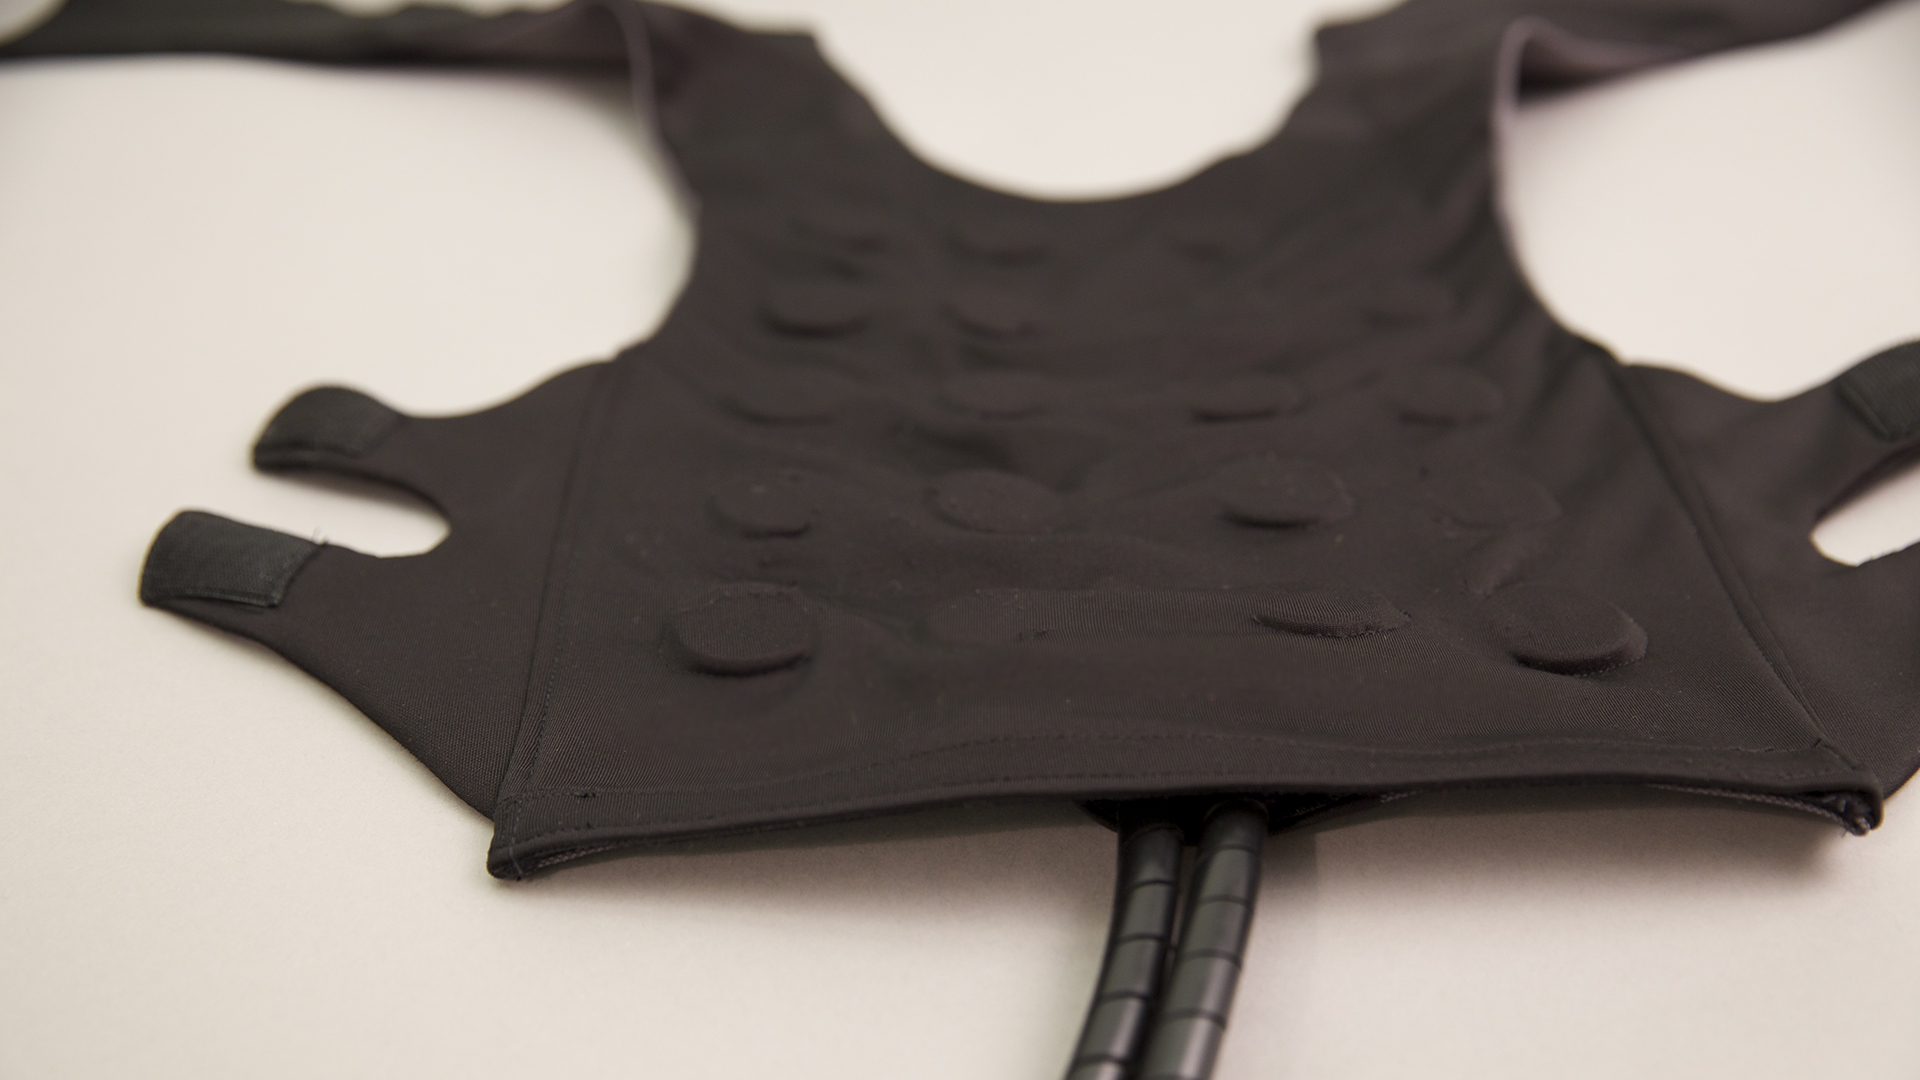
\includegraphics[width=\textwidth]{vest4} 
%	   \caption{Vest}
%	   \label{fig:devices:vest}
%    \end{subfigure}
%     \begin{subfigure}[b]{0.235\textwidth}
%	   	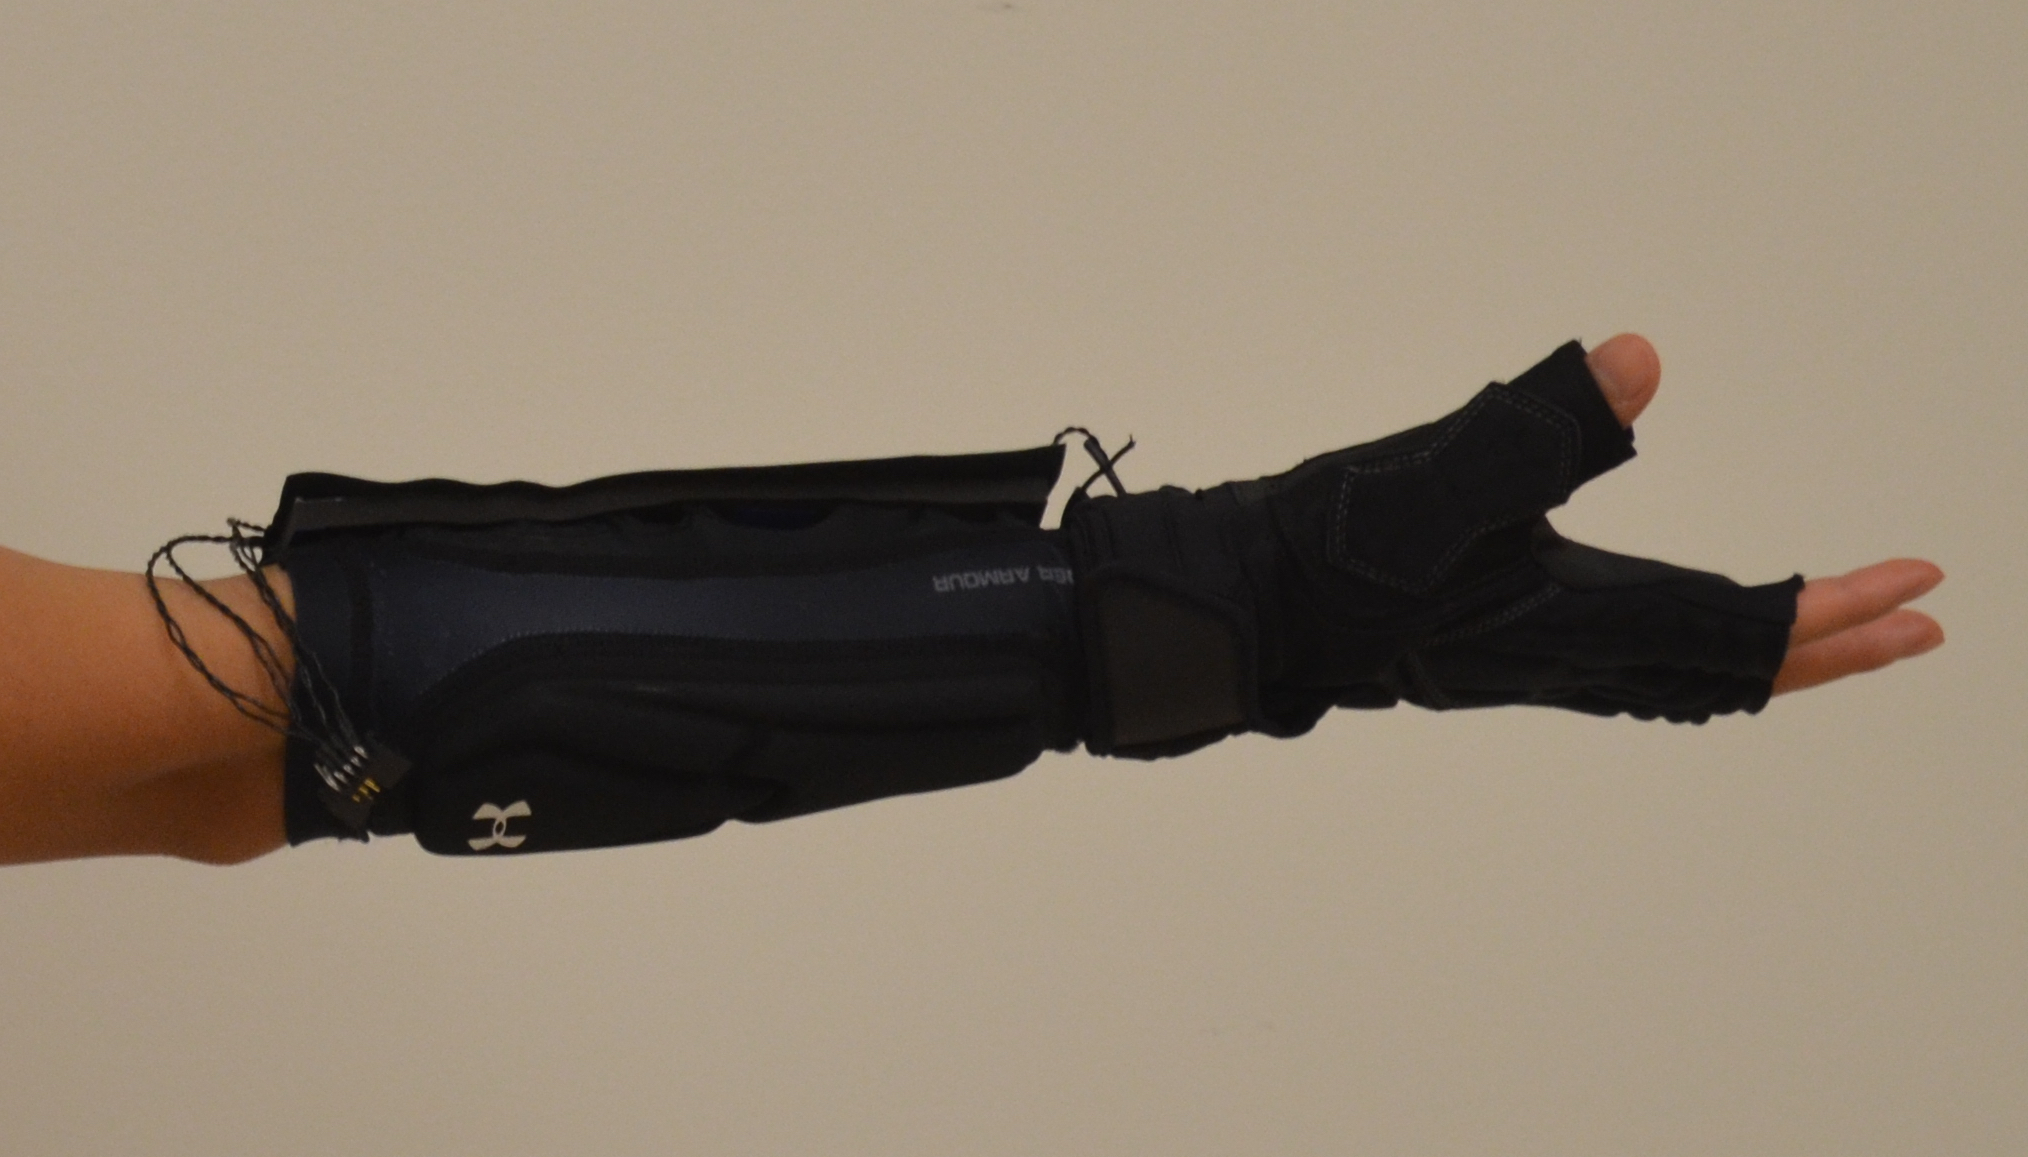
\includegraphics[width=\textwidth]{glove} 
%	   \caption{Glove}
%	   \label{fig:devices:glove}
%    \end{subfigure}
%    	   \caption{Other supported devices.}
%	   \label{fig:devices}
%\end{figure}


%\begin{figure}[htb] %  figure placement: here, top, bottom, or page
%   \centering
%	   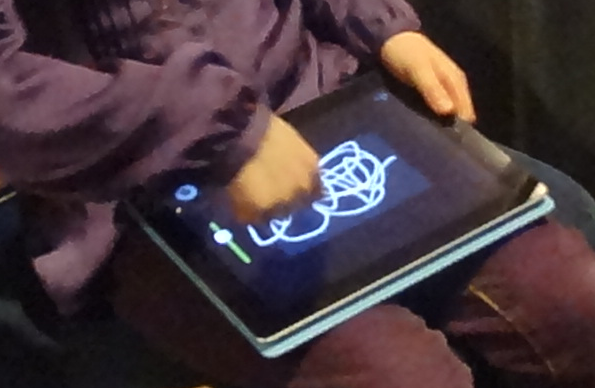
\includegraphics[width=0.47\textwidth]{tablet-input} 
%        	   \caption{Tactile animation objects implemented on a tablet.}
%	   \label{fig:tabletinput}
%\end{figure}



\subsection{Limitations}
While the tactile animation metaphor seems promising and may apply to many contexts, it is limited by the requirement of a suitable rendering algorithm for target hardware.
We have not yet explored other form factors, such as handhelds, multi-device scenarios, or non-vibrotactile sensations.
Although we perceptually optimized our algorithm, we did not conduct a full psychophysical investigation.
Further work needs to be done to identify the limits, thresholds, and peculiarities of this rendering technique.
Examples include:
curved trajectories of animation objects (although participants' use of curved motion was encouraging, e.g., P5's turn left sensation),
spatial frequency control (how to superpose animation objects of differing frequencies),
non-triangular meshes (e.g., quadrilateral interpolation or kernel methods),
and mixed actuator types (such as a chair with both voice coil and rumble motors, \autoref{fig:application:space}e).

%%%%%%%%%%
%
%Implications for Design
%
%%%%%%%%%%
\section{Conclusion}

%This paper presents Mango, a new tactile animation tool to create rich, dynamic and expressive haptic experiences. 
%The tool utilizes animation metaphor in the design process and renders animated VT patterns on a variety of spatial VT displays.
%Design requirements gathered in interviews and literature review are implemented on a prototype software that was evaluated with artists and a normal everyday computer user.
%The post evaluation interviews and feedback suggested that the tool was useful and easily adaptable; and participants highly preferred animation metaphor to design haptic patterns.
%Overall, tactile animation represents a promising new direction to support haptic media design.

%A key feature of Mango is that it can be used with a wide range of haptic feedback hardware. The hardware specific definitions are provided in the configuration file which facilitates authoring of animations and its rendering on the hardware. Configuration files for new hardware can be constructed and loaded in Mango, to use its authoring capabilities with new hardware.  

%\kmC{Adjust weight: tactile animation then Mango} % Km: up to here, I think it's consistent now. I ran out of steam.
This paper introduces the \emph{tactile animation object}, a new abstraction for creating rich and expressive haptic media on grid displays.
% The design of Mango is derived from an
This animation metaphor allows designers and media artists to directly manipulate phantom vibrotactile sensations continuously in both space and time.
Our rendering pipeline, which uses a perceptually-guided phantom sensation algorithm, enables critical real-time feedback for designing.
%an approach that is more direct and potentially creative than coordinating individual actuators, and which scales better to large actuator maps, where perceived motion is nearly intractable using track-based approaches.
%Unlike previous tools that either required rigorous programming background or was applicable to a specific hardware configuration, an animation approach also % our tool
%provides a familiar interface to a large animation workforce, therefore eliminating training time and cost necessary for haptic content production in the mainstream media.  
We incorporated these ideas into a prototype, Mango, with a design grounded in animator requirements and haptic design guidelines.
Professional animators used our tool to create a variety of designs, giving positive feedback and excitement for future versions.
This approach has the potential to % KM: concerned that this functionality can be added to any tool with properly designed configuration files, and isn't tied particularly to the other innovations reported here. If so, need to be much more careful about how it's phrased since this capability isn't even really demonstrated here - you only use one display apparatus.
% Moreover, Mango 
accommodate a large variety of haptic hardware, ranging from a single shaking element mounted on the seat to an array of actuators stimulating multiple points on the skin, and can export content into formats applicable in the production pipeline.
Tactile animation empowers animators with a new set of artistic tools for rich, multimodal feedback. 

\section{Acknowledgments}
We thank our reviewers and participants for their valuable feedback.
This work was supported by Disney Research, with
additional support provided by NSERC.
%Oliver holds an NSERC CGS D scholarship.


%
%
%\subsection{Demo}
%\osC{Add image, description, takeaway from demo}
%
%\section{Discussion}
%The Tactile Animation project expanded our understanding from the Haptic Instrument study in \autoref{ch:hapticinstrument}.
%Specifically, it reaffirmed the value of real-time feedback and the need for examples, and showed that a persistent object model reduces cognitive load.
%It also suggests again that examples and user experiences are extremely valuable to the design process, providing motivation for example-based haptic design discussed next in \autoref{ch:hapticexamples}.
%
%
%
\endinput
